\documentclass[11pt]{book}
\pagestyle{plain}
%\documentclass{article}
\usepackage[utf8]{inputenc}
\usepackage[english]{babel}
\usepackage{latexsym,amsmath,amssymb}
\usepackage{amsthm}
%\usepackage[notref,notcite]{showkeys}
\usepackage{amsfonts}
\usepackage{geometry}
\usepackage{graphicx}
\usepackage{lmodern}
\usepackage{pifont}
\usepackage{tikz}
\usepackage{pgfplots}
\usepackage{thmtools}
\usepackage{wrapfig}
\usepackage{extarrows}
\usepackage{breqn}
\usepackage{physics}
\usepackage{afterpage}
%\usepackage{enumitem}
\usepackage[inline]{enumitem}
\usepackage{mathrsfs}
\usepackage{scalerel}
\usepackage{stackengine,wasysym}
\usepackage{aligned-overset}
\usepackage{stackengine}
\usepackage{mathtools}
\usepackage{nccmath}
\usepackage{url}
\usepackage{float}
\usepackage{lipsum}
\usepackage[toc]{appendix}
\usepackage{chngcntr}
\usepackage{etoolbox}
\usepackage{framed}
\usepackage{mdframed}
\usepackage{blindtext}
\usepackage{xcolor}
\usepackage{fancyhdr}
\usepackage{titlesec}
\graphicspath{{images/}}

\titleformat{\chapter}[block]{\huge\bfseries\itshape}{\chaptertitlename\  \thechapter.}{0.5ex}{}[]

\titleformat{\section}[block]{\Large\bfseries\itshape}{\thesection}{0.5ex}{}[]

\titleformat{\subsection}[block]{\large\bfseries\itshape}{\thesubsection}{0.5ex}{}[]

\usepackage{hyperref}
\hypersetup{
    colorlinks = true,
    linkcolor = blue,
    filecolor = blue,      
    urlcolor = blue,
    citecolor = blue,
    pdftitle = {Sharelatex Example},
    bookmarks = true,
    pdfpagemode = FullScreen,
}

\urlstyle{same}

\newcommand*\circled[1]{\tikz[baseline=(char.base)]{
            \node[shape=circle,draw,inner sep=2pt] (char) {#1};}}

\setlength{\oddsidemargin}{1pt}
\setlength{\evensidemargin}{1pt}
\setlength{\marginparwidth}{30pt} % these gain 53pt width
\setlength{\topmargin}{1pt}       % gains 26pt height
\setlength{\headheight}{1pt}      % gains 11pt height
\setlength{\headsep}{1pt}         % gains 24pt height
%\setlength{\footheight}{12 pt} 	  % cannot be changed as number must fit
\setlength{\footskip}{24pt}       % gains 6pt height
\setlength{\textheight}{650pt}    % 528 + 26 + 11 + 24 + 6 + 55 for luck
\setlength{\textwidth}{460pt}     % 360 + 53 + 47 for luck

\title{Sections and Chapters}

\newtheorem{definition}{Definition}[chapter]
\newtheorem{theorem}{Theorem}[chapter]
\newtheorem{corollary}{Corollary}[theorem]
\newtheorem{lemma}[theorem]{Lemma}
\newtheorem{proposition}{Proposition}[chapter]
\newtheorem{exercise}{Exercise}[chapter]
\newtheorem{remark}{Remark}[chapter]
\theoremstyle{definition}
\newtheorem{example}{Example}[chapter]
\numberwithin{equation}{chapter}


\AtBeginEnvironment{subappendices}{%
\Appendix*{Appendix}
\addcontentsline{toc}{chapter}{Appendices}
\counterwithin{figure}{section}
\counterwithin{table}{section}
}

\newmdenv[
  linewidth=1.5pt, 
  topline=false, 
  bottomline=false, 
  rightline=false,
  innerleftmargin=15pt,
  leftmargin=10pt,
  rightmargin=0pt,
  innerrightmargin=0pt, 
]{claim}

\def\MM{\mathfrak{M}}
\def\BB{\mathfrak{B}}
\def\CC{\mathfrak{C}}
\def\leb{{\mathcal L}}
\def\H{{\mathcal H}}
\def\L{{\mathcal L}}

\pagestyle{fancy}
\fancyhf{}
\fancyhead[LE]{{\em \thepage}}
\fancyhead[RE]{{\em \leftmark}}
\fancyhead[LO]{{\em \rightmark}}
\fancyhead[RO]{{\em \thepage}}

\counterwithout{footnote}{chapter}

\def\dsp{\def\baselinestretch{1.35}\large
\normalsize}
%%%%This makes a double spacing. Use this with 11pt style. If you
%%%%want to use this just insert \dsp after the \begin{document}
%%%%The correct baselinestretch for double spacing is 1.37. However
%%%%you can use different parameter.

\newcommand\blankpage{%
    \null
    \thispagestyle{empty}%
    \addtocounter{page}{-1}%
    \newpage}
    
\def\U{{\mathcal U}}

\begin{document}
\frontmatter

\begin{titlepage}
	\begin{center}
	\textbf{\LARGE{}} \\
	\vspace{40mm}
    \textbf{\Huge{Analysis}} \\
    \medskip
    \vspace{2mm} %5mm vertical space
    \large{\textsc{Zhen Yao}}\\
    %\large{\textsc{University of Pittsburgh}}
    \end{center}
\end{titlepage}

\tableofcontents{}
\mainmatter

\newpage

\chapter{Measure Theory}

Let $A \subset X$ be a subset of $X$, and we want to assign {\em measure} $\mu(A)$ to this set. Denote by $\MM \subset P(X)$ the class of sets for which the measure $\mu$ is defined, where $P(X)$ is the power set of $X$, that is the set of all subsets of $X$. Elements of $\MM$ are called {\em measurable sets}. What properties do we need to define measure?
\begin{enumerate}[label=(\alph*)]
    \item $X \subset \MM$;
    
    \item If $A \in \MM$, then $X \setminus A \in \MM$;
    
    \item If $A_1, A_2, \cdot \in \MM$, then $\bigcup^\infty_{i=1}A_i \in \MM$.
\end{enumerate}

\medskip

\section{$\sigma$-algebra}

\begin{definition}\label{definition_sigma_algebra}
Let $X$ be a set. A collection $\MM$ of subsets of $X$ is $\sigma$-algebra if $\MM$ has the following properties:
\begin{enumerate}[label=(\alph*)]
    \item $X \in \MM$;
    
    \item If $A \in \MM$, then $X \setminus A \in \MM$;
    
    \item If $A_1, A_2, \cdots \in \MM$, then $\bigcup^\infty_{i=1}A_i \in \MM$.
\end{enumerate}
Then the $(X,\MM)$ is called measurable space and elements of $\MM$ are called measurable sets.
\end{definition}

\medskip

\begin{exercise}\label{exercise_11} {\rm \cite{1}}
Let $(X, \MM)$ be a measurable space. Show that
\begin{enumerate}[label=(\alph*)]
    \item $\emptyset \in \MM$;
    
    \item $A, B \in \MM$, then $A \setminus B \in \MM$;
    
    \item $\MM$ is closed under finite and countable unions and intersections.
\end{enumerate}
\end{exercise}
\begin{proof}
~\begin{enumerate}[label=(\alph*)]
    \item $\emptyset = X \setminus X$, then $\emptyset \in \MM$.
   
    \item By Definition \ref{definition_sigma_algebra}(c), $A \cup B \cup \emptyset \cup \emptyset \cup \cdots \in \MM$, which implies $A \cup B \in \MM$. 
    
    By De Morgan's Laws, we have 
    \begin{align*}
        X \setminus (A \cap B) = (X \setminus A) \cup (X \setminus B),
    \end{align*}
    and since $X \setminus A, X \setminus B \in \MM$, $A \cap B \in \MM$.
    
    Now, $A \setminus B = A \cap (X \setminus B)$, then by the results above, we have $A \setminus B \in \MM$.
    
    \item Suppose $A_1, A_2, \cdots \in \MM$, by De Morgan's Laws, we have
    \begin{align*}
        X \setminus \bigcap^\infty_{i=1} A_i = \bigcup^\infty_{i=1} (X \setminus A_i),
    \end{align*}
    and since $X \setminus A_i \in \MM$, then $X \setminus \bigcap^\infty_{i=1} A_i \in \MM$, and thus $\bigcap^\infty_{i=1} A_i \in \MM$. 
\end{enumerate}
\end{proof}

\medskip

\begin{example}[Examples of $\sigma$-algebra]
~\begin{enumerate}[label=(\alph*)]
    \item $P(X)$, or $2^X$, the family of all subsets of $X$ is a $\sigma$-algebra.
    
    \item $\MM = \{\emptyset, X\}$ is a $\sigma$-algebra.
    
    \item If $E \subset X$ is a fixed set, then $\MM = \{\emptyset, X, E, X\setminus E\}$ is a $\sigma$-algebra.
\end{enumerate}
\end{example}

\medskip

\begin{proposition}\label{prop_11}
A family $\MM$ of subsets of $X$ is a $\sigma$-algebra if and only if
\begin{enumerate}[label=(\alph*)]
    \item $X \in \MM$;
    
    \item If $A,B \in \MM$, then $A \setminus B \in \MM$;
    
    \item If $A_1, A_2, \cdots \in \MM$ are pairwise disjoint, then $\bigcup^\infty_{i=1} A_i \in \MM$.
\end{enumerate}
\end{proposition}
\begin{proof} 
~\begin{enumerate}
    \item[($\Rightarrow$)] (a) and (c) are obvious, it remains to show (b). By definition of $\sigma$-algebra, $A \cup B \cup \emptyset \cup \emptyset \cup \cdots \in \MM$, which implies $A \cup B \in \MM$. Also, by De Morgan's Laws, we have 
    \begin{align*}
        X \setminus (A \cap B) = (X \setminus A) \cup (X \setminus B),
    \end{align*}
    and since $X \setminus A, X \setminus B \in \MM$, $A \cap B \in \MM$. Now, $A \setminus B = A \cap (X \setminus B)$, then by the results above, we have $A \setminus B \in \MM$.
    
    \item[($\Leftarrow$)] It suffices to show that for any $A_1, A_2,\cdots \in \MM$, $\bigcup^\infty_{i=1}A_i \in \MM$. Let $B_1 = A_1$, $B_2 = A_2 \setminus A_1$, $B_3 = A_3 \setminus (B_1 \cup B_2)$ and so on. It gives a pairwise disjoint sequence of sets $B_1, B_2, \cdots \in \MM$. By the assumption, $\bigcup^\infty_{i=1}A_i = \bigcup^\infty_{i=1}B_i \in \MM$.
\end{enumerate}
\end{proof}

\medskip

\begin{proposition}
If $\{\MM_i\}_{i\in I}$ is a family of $\sigma$-algebras, then
\begin{align*}
    \MM = \bigcap_{i \in I} \MM_i
\end{align*}
is a $\sigma$-algebra. Note that $I$ can be uncountable.
\end{proposition}
\begin{proof}
~\begin{enumerate}[label=(\alph*)]
    \item For any $i \in I$, $\emptyset \in \MM_i$, then $\emptyset \in \bigcap_{i \in I} \MM_i$.
    
    \item If $A_i \in \bigcap_{i \in I} \MM_i$, then $A_i \in \MM_i$ for all $i \in I$, which implies $X\setminus A_i \in \MM_i$ for all $i \in I$. Hence, $X\setminus A_i \in \bigcap_{i \in I} \MM_i$.
    
    \item For $A_j \in \bigcap_{i \in I} \MM_i$, $j = 1, 2, \cdots$, it means that for all $j = 1, 2, \cdots$ and all $i \in I$, $A_j \in \MM_i$, and then for all $i \in I$, $\bigcup^\infty_{j=1} A_j \in \MM_i$. Thus, $\bigcup^\infty_{j=1} A_j \in \bigcap_{i \in I} \MM_i$.
\end{enumerate}

\end{proof}


\medskip

Let $\mathcal{R}$ be a family of subsets of $X$. Denote by $\sigma(\mathcal{R})$ the intersection of all $\sigma$-algebras that contain $\mathcal{R}$. Note that there is at least one $\sigma$-algebra that contains $\mathcal{R}$, namely the power set $P(X)$. We say that $\sigma(\mathcal{R})$ a {\em $\sigma$-algebra generated by $\mathcal{R}$}. Also, $\sigma(\mathcal{R})$ is the {\em smallest} $\sigma$-algebra that contains $\mathcal{R}$ in the sense that if $\MM$ is a $\sigma$-algebra that contains $\mathcal{R}$, then $\sigma(\mathcal{R}) \subset \MM$.

\medskip

\begin{example}
If $\mathcal{R} = \{E\}$, then $\sigma(\mathcal{R}) = \{\emptyset, X, E, X\setminus E\}$.
\end{example}

\medskip

\begin{theorem}{\rm \cite{2}}
If $\mathcal{R}$ is any collection of subsets of $X$, there exists a smallest $\sigma$-algebra $\sigma(\mathcal{R})$ in $X$ such that $\mathcal{R} \in \sigma(\mathcal{R})$.
\end{theorem}
\begin{proof}
Let $\Omega$ be the family of all $\sigma$-algebras $\MM$ in $X$ that contains $\mathcal{R}$. Since
the collection of all subsets of $X$ is such a $\sigma$-algebra, then $\Omega$ is not empty. Let $\MM^*$ be the intersection of all $\MM \in \Omega$. It is clear that $\mathcal{R} \subset \MM^*$ and that $\MM^*$ lies in every $\sigma$-algebra in $X$ which contains $\mathcal{R}$. It suffices to show that $\MM^*$ is itself a $\sigma$-algebra.

If $A_n \in \MM^*$ for $n = 1,2,3,\cdots$, and it $\MM \in \Omega$, then $A_n \in \MM$, so $\bigcup A_n \in \MM$, since $\MM$ is a $\sigma$-algebra. Since $\bigcup A_n \in \MM$ for every $\MM \in \Omega$, we conclude that $\bigcup A_n \in \MM^*$.
\end{proof}

\medskip


\section{Borel sets}

\begin{definition}
Let $X$ be a metric space (or topological space). Denote by $\mathfrak{B}(X)$ the $\sigma$-algebra generated by the family of all open sets in $X$. Elements of $\mathfrak{B}(X)$ are called Borel sets and $\mathfrak{B}(X)$ is called $\sigma$-algebra of Borel sets. So,
\begin{enumerate}[label=(\alph*)]
    \item All closed sets are Borel sets;
    
    \item If $G_1, G_2, \cdots$ are open, then $\bigcap^\infty_{i=1}G_i$ is Borel, and such sets are called $G_\delta$ sets.
    
    \item If $F_1, F_2, \cdots$ are closed, then $\bigcup^\infty_{i=1}F_i$ is Borel, and such sets are called $F_\sigma$ sets.
\end{enumerate}
The notations $G_\delta$ and $F_\sigma$ is due to Hausdorff{\rm \cite{2}}.
\end{definition}

\medskip

\begin{example}
Every closed set is $G_\delta$. Indeed, suppose $F$ is closed, and let
\begin{align*}
    G_i = \left\{x\,|\, \operatorname{dist}(x,F) < \frac{1}{i}\right\},
\end{align*}
where $G_i$ are open, and then $F = \bigcap^\infty_{i=1} G_i$.

Similarly, every open set is $F_\sigma$. Suppose $G$ is open set, and let $F = X \setminus E$, which is closed. Then,
\begin{align*}
    G = X \setminus F = X \setminus \bigcap^\infty_{i=1} G_i = \bigcup^\infty_{i=1} (X \setminus G_i),
\end{align*}
where $X \setminus G_i$ are closed.
\end{example}

\medskip

\begin{proposition}
Let $A \subset X$. $A$ is $F_\sigma$ set if and only if $X \setminus A$ is $G_\delta$.
\end{proposition}
\begin{proof}
~\begin{enumerate}[label=(\alph*)]
    \item ($\Rightarrow$) By assumption, $A = \bigcup^\infty_{i=1} F_i$, where $F_i$ are closed. Then, $X \setminus A = \bigcap^\infty_{i=1} (X \setminus F_i)$, where $X \setminus F_i$ are open. This implies $X \setminus A$ is $G_\delta$.
    
    \item ($\Leftarrow$) This direction is similar.
\end{enumerate}
\end{proof}

\medskip

\begin{example}
$\mathbb{Q}$ is a $F_\delta$ set, where $\mathbb{Q}$ is the set of all rational number.
\end{example}
\begin{proof}
Since $\mathbb{Q}$ is countable, we could write it as $\mathbb{Q} = \{q_1, q_2, \cdots\}$, and it is obvious that $\mathbb{Q} = \bigcup^\infty_{i=1} \{q_i\}$, where $\{q_i\}$ is closed. Thus, $\mathbb{Q}$ is $F_\delta$.
\end{proof}

\medskip

\begin{theorem}[{\bf Baire Category}]
Let $X$ be a complete metric space, $G_i \subset X, i = 1,2,\cdots$ are open and dense in $X$. Then, $\bigcap^\infty_{i=1} G_i$ is also dense.
\end{theorem}
\begin{proof}
The proof is from Rudin's {\em Real and Complex Analysis}\cite{2}. Let $W$ be any open set in $X$, a subset is dense if and only if every nonempty open subset intersects it. Thus, to show that the intersection is dense it suffice to show that $\bigcap^\infty_{i=1} G_i$ has a point in $W$ if $W \neq \emptyset$.

Since $G_1$ is dense, then $G_1 \cap W \neq \emptyset$, then there is a point $x_1$ and $0 < r_1 < 1$ such that
\begin{align}\label{Baire_Category_1}
    \overline{B}\left(x_1,r_1\right) \subset (G_1 \cap W),
\end{align}
where $\overline{B}(x,r)$ denotes the closure of $B(x,r)$. Since each $G_i$ is dense, continuing this process gives sequences $\{x_n\} \in X$ and $\{r_n\}$ such that 
\begin{align}\label{Baire_Category_2}
    B\left(x_n,r_n\right) \subset \left( B\left(x_{n-1},r_{n-1}\right) \cap G_n \right), \quad 0 < r_n < \frac{1}{n}.
\end{align}
Then, for $n > m$, we have $x_n \in B(x_m,r_m)$, and hence $\{x_n\}$ is a Cauchy sequence. By completeness of $X$, there exists some point $x$ in $X$ such that $\lim_{n\to\infty} x_n = x$.

Since $x_n \in \overline{B}(x_m,r_m)$ for $n > m$, then $x \in \overline{B}(x_n,r_n)$ for each $n \in \mathbb{N}$ and by (\ref{Baire_Category_2}), $x \in G_i$ for $i = 1,2,\cdots$. By (\ref{Baire_Category_1}), $x \in W$, and thus $\bigcap^\infty_{i=1} G_i$ is dense. 
\end{proof}

\medskip

\begin{example}
$\mathbb{Q}$ is not a $G_\sigma$ set, i.e. $\mathbb{Q} \in F_\delta \setminus G_\sigma$.
\end{example}
\begin{proof}
Suppose $\mathbb{Q}$ is $G_\sigma$, then $\mathbb{Q} = \bigcap^\infty_{i=1} G_i$, where $G_i$ is dense in $\mathbb{R}$. Let $\widetilde{G_i} = \mathbb{R} \setminus \{q_i\}, q_i \in \mathbb{Q}$ for $i = 1,2,\cdots$, which are open and dense. Now,
\begin{align*}
    \left(\bigcap^\infty_{i=1}G_i\right) \cap \left(\bigcap^\infty_{i=1}\widetilde{G_i}\right) = \mathbb{Q} \cap (\mathbb{R} \setminus \mathbb{Q}) = \emptyset,
\end{align*}
and this is a contradiction to Baire Category theorem.
\end{proof}

\medskip

Now what are Borel sets? Recall that open, closed sets, $G_\delta, F_\sigma$, intersections of countable many $F_\sigma$'s and union of countable many $G_\delta$'s are all in Borel sets $\mathfrak{B}(X)$, but these are only a small part of Borel sets. We need well-ordering and ordinal numbers\footnote{See Appendix \ref{appendix_a}.} to introduce Borel hierarchy, and then to construct Borel sets.

\medskip


Let's introduce the {\em finite Borel hierarchy}.

\begin{definition}[{\bf Borel sets of finite order}]
Let
\begin{align*}
    \Sigma_1 & = \{G\,|\, G \subseteq X, G\,\, \text{is open}\}, \\
    \Pi_1 & = \{F\,|\, F \subseteq X, F\,\, \text{is closed}\},
\end{align*}
and then inductively define the following collection of subsets of $X$
\begin{align*}
    \Sigma_{n+1} & = \left\{\bigcup^\infty_{i=1} F_i \,|\, F_i \in \Pi_{n}\right\}, \\
    \Pi_{n+1} & = \left\{\bigcup^\infty_{i=1} G_i \,|\, G_i \in \Sigma_{n}\right\}.
\end{align*}
\end{definition}

\medskip

\begin{theorem}
~\begin{enumerate}[label=(\alph*)]
    \item If $S \subset \mathbb{R}$, then $S \subset \Sigma_{n}$ if and only if $\mathbb{R} \setminus S \in \Pi_{n}$.
    
    \item For any $n \in \mathbb{N}$, $\Sigma_{n} \subset \Sigma_{n+1}$, $\Pi_{n} \in \Pi_{n+1}$ and $\Sigma_{n} \in \Pi_{n+1}$, $\Pi_{n} \in \Sigma_{n+1}$. Also, 
    \begin{align*}
        \left(\Pi_{n} \cap \Sigma_{n}\right) \subset \left(\Pi_{n+1} \cap \Sigma_{n+1}\right).
    \end{align*}
\end{enumerate}
\end{theorem}

\medskip

\begin{definition}
Let $B \subset \mathbb{R}$ be a Borel set. $B$ has Borel rank $n \in \mathbb{N}$ if $n$ is the least integer such that $$B \subset \left(\Sigma_n \cup \Pi_n \right) \setminus \left(\Sigma_{n-1} \cap \Pi_{n-1}\right).$$
\end{definition}

\medskip

\begin{example}
Open and closed subset of $\mathbb{R}$ has Borel rank $1$, $\mathbb{Q}$ has Borel rank $2$.
\end{example}

\medskip

\begin{theorem}
There are Borel sets of infinite rank.
\end{theorem}

\medskip

We considered all Borel sets of finite rank, but how to construct a set belong to $\mathfrak{B}(X)$ but with infinite rank?

Let $S_n \subset (n,n+1)$ with Borel rank $n$, then $S_1 \cup S_2 \cup \cdots$ is also Borel but with infinite rank. Now let $\Sigma_\omega$ be the unions of Borel sets of finite rank, and $\Pi_\omega$ be the intersections of Borel sets of finite rank. And we can define $\Sigma_{\omega+1}$ and $\Pi_{\omega+1}$ accordingly. 

\medskip

\begin{theorem}
$\mathfrak{B}(\mathbb{R}) = \bigcup (\Sigma_\omega \cup \Pi_\omega)$, where $\omega$ is countable, ordinal number.
\end{theorem}

\medskip

\section{Measure}

\begin{definition}
Let $(X, \MM)$ be a measurable space. A measure (also called positive measure) is a function $\mu: \MM \to [0,\infty]$ such that
\begin{enumerate}[label=(\alph*)]
    \item $\mu(\emptyset) = 0$;
    
    \item $\mu$ is countably additive, i.e. if $A_1, A_2, \cdots \in \MM$ are pairwise disjoint, then
    \begin{align*}
        \mu \left( \bigcup^\infty_{i=1} A_i \right) = \sum^\infty_{i=1} \mu(A_i).
    \end{align*}
\end{enumerate}
And ``ordered triples'' $(X, \MM, \mu)$ is called a measure space. If $\mu(X) < \infty$, then $\mu$ is called finite measure. If $\mu(X) = 1$, then $\mu$ is called probability or probability measure. If $X = \bigcup^\infty_{i=1} A_i$, where $A_i \in \MM$ and $\mu(A_i) < \infty$ for all $i = 1,2,\cdots$, then we say $\mu$ is $\sigma$-finite. 
\end{definition}

\medskip

\begin{example}
If $X$ is an arbitrary set, and $\mu: P(X) \to [0,\infty]$ is defined by $\mu(E) = m$ if $E$ is finite and has $m$ elements, $\mu(E) = \infty$ if $E$ is infinite, then $\mu$ is a measure and called {\em counting measure}.
\end{example}

\begin{theorem}[{\bf Elementary properties of measures}]\label{theorem_111}
Let $(X, \MM, \mu)$ be a measure space. Then
\begin{enumerate}[label=(\alph*)]
    \item If the sets $A_1, A_2, \cdots, A_n \in \MM$ are pairwise disjoint, then $\mu \left(\bigcup^n_{i=1} A_i \right) = \sum^n_{i=1} \mu(A_i)$.
    
    \item If $A, B \in \MM$, $A \subset B$, then $\mu(A) \leq \mu(B)$.
    
    \item If $A, B \in \MM$, $A \subset B$, $\mu(B) < \infty$, then $\mu(B\setminus A) = \mu(B) - \mu(A)$.
    
    \item If $A_1, A_2, \cdots \in \MM$, then 
    \begin{align*}
        \mu \left(\bigcup^\infty_{i=1} A_i \right) \leq \sum^\infty_{i=1} \mu(A_i).
    \end{align*}
    
    \item If $A_1, A_2, \cdots \in \MM$, $\mu(A_i) = 0$ for $i = 1,2,\cdots$, then $\mu \left(\bigcup^\infty_{i=1} A_i \right) = 0$.
    
    \item If $A_1, A_2, \cdots \in \MM$, $A_1 \subset A_2 \subset \cdots$, then
    \begin{align*}
        \mu \left(\bigcup^\infty_{i=1} A_i \right) = \lim_{i\to\infty} \mu(A_i).
    \end{align*}
    
    \item If $A_1, A_2, \cdots \in \MM$, $A_1 \supset A_2 \supset \cdots$ and $\mu(A_1) < \infty$, then
    \begin{align*}
        \mu \left(\bigcap^\infty_{i=1} A_i \right) = \lim_{i\to\infty} \mu(A_i).
    \end{align*}
\end{enumerate}
\end{theorem}
\begin{proof}
~\begin{enumerate}[label=(\alph*)]
    \item Considering the sequence $A_1, A_2, \cdots, A_n, \emptyset, \emptyset, \cdots$, which are pairwise disjoint, then by definition of measure, \begin{align*}
        \mu(A_1 \cup A_2 \cup \cdots \cup A_n) & = \mu(A_1) + \cdots + \mu(A_n) + \mu(\emptyset) + \cdots + \mu(\emptyset) \\
        & = \mu(A_1) + \cdots + \mu(A_n).
    \end{align*}
    
    \item Since $B = A \cup (B)$ and $A \cap (B \setminus A) = \emptyset$, then $\mu(B) = \mu(A) + \mu(B \setminus A) \geq \mu(A)$.
    
    \item By $\mu(B) = \mu(A) + \mu(B \setminus A)$ in (b). Note that we need $\mu(B) < \infty$. Otherwise, it could happen that $\mu(A) = \mu(B) = \infty$ and then $\mu(B \setminus A) = \mu(B) - \mu(A) = \infty - \infty$.
    
    \item Since
    \begin{align*}
        \bigcup^\infty_{i=1} A_i = \underbrace{A_1}_{B_1} \cup \underbrace{(A_2\setminus A_1)}_{B_2} \cup \underbrace{(A_3 \setminus (A_1\cup A_2))}_{B_3} \cup \cdots,
    \end{align*}
    and $B_1, B_2, \cdots$ are pairwise disjoint, then 
    \begin{align}\label{equaiton_11}
        \mu(A) = \sum^\infty_{i=1} \mu(B_i) \leq \sum^\infty_{i=1} \mu(A_i).
    \end{align}
    
    \item It follows from (\ref{equaiton_11}).
    
    \item Since $A_i \subset A_{i+1}$, then 
    \begin{align*}
        \bigcup^\infty_{i=1} A_i =  \underbrace{A_1}_{B_1} \cup \underbrace{(A_2\setminus A_1)}_{B_2} \cup \underbrace{(A_3 \setminus A_2)}_{B_3} \cup \underbrace{(A_4 \setminus A_3)}_{B_4} \cup \cdots,
    \end{align*}
    and $B_i$ are pairwise disjoint. Therefore,
    \begin{align*}
        \mu \left(\bigcup^\infty_{i=1} A_i \right) = \sum^\infty_{i=1} \mu(B_i) = \lim_{i\to\infty} \sum^i_{k=1} \mu(B_k) = \lim_{i\to\infty} \mu \left(\bigcup^i_{k=1} B_k \right) = \lim_{i\to\infty} \mu(A_i).
    \end{align*}
    The limit exists because $\mu(A_i) \leq \mu(A_{i+1})$.
    
    \item Apply (f) to the sets $A_1\setminus A_i$. Let $C_i = A_1 \setminus A_i$, then $C_1 \subset C_2 \subset \cdots$ and $\mu(C_i) = \mu(A_1) - \mu(A_i)$. Also, $A \setminus \left( \bigcap^\infty_{i=1} A_i\right) = \bigcup^\infty_{i=1} C_i$, then by (f), we have
    \begin{align*}
        \mu(A_1) - \mu \left(\bigcap^\infty_{i=1} A_i\right) = \mu\left(A_1 \setminus \bigcap^\infty_{i=1} A_i\right) = \lim_{i\to\infty} \mu(C_i) = \mu(A_1) - \lim_{i\to\infty} \mu(A_i),
    \end{align*}
    and this is where we used the fact that $\mu(A_1) < \infty$.
\end{enumerate}
\end{proof}

\medskip

\section{Outer measure and Carathéodory construction}

Constructing a measure with desired properties is difficult, but it is much easier to construct {\em outer measure}, since it has less restrictive properties. Then the Carathéodory theorem shows how to construct a measure from an outer measure.

\medskip

\begin{definition}
Let $X$ be a set. A function $\mu^*: P(X) \to [0,\infty]$ is called outer measure if 
\begin{enumerate}[label=(\alph*)]
    \item $\mu^*(\emptyset) = 0$;
    
    \item If $A \subset B$, the $\mu^*(A) \leq \mu^*(B)$;
    
    \item For all sets $A_1, A_2, \cdots \subset X$,
    \begin{align*}
        \mu^* \left( \bigcup^\infty_{i=1} A_i \right) \leq \sum^\infty_{i=1} \mu^*(A_i).
    \end{align*}
\end{enumerate}
\end{definition}

\medskip

\begin{definition}
A set $E$ is said to be $\mu^*$-measurable if for all $A \subset X$,
\begin{align}\label{equation_14}
    \mu^*(A) = \mu^*(A \cup E) + \mu^*(A \setminus E).
\end{align}
Condition (\ref{equation_14}) is called Carathéodory condition.
\end{definition}

\begin{remark}
The inequality 
\begin{align*}
    \mu^*(A) \leq \mu^*(A \cup E) + \mu^*(A \setminus E)
\end{align*}
always holds. In order to verify measurability of a set $E$, it suffices to show that 
\begin{align*}
    \mu^*(A) \geq \mu^*(A \cup E) + \mu^*(A \setminus E).
\end{align*}
\end{remark}

\medskip

\begin{proposition}\label{prop_14}
All sets with $\mu^*(E) = 0$ are $\mu^*$-measurable.
\end{proposition}
\begin{proof}
If $\mu^*(E) = 0$, then for an arbitrary set $A \subset X$, we have
\begin{align*}
    \mu^*(A) \geq \mu^*(A \setminus E) = \mu^*(A \setminus E) + \underbrace{\mu^*(A \cap E)}_{0},
\end{align*}
where the last term follows from $(A \cap E) \subset E$.
\end{proof}

\medskip

\begin{definition}
Let $\MM^*$ be the class of all $\mu^*$-measurable sets.
\end{definition}

\medskip

\begin{theorem}[{\bf Carathéodory}]\label{caratheodory_theorem}
$\MM^*$ is a $\sigma$-algebra and $\mu^*: \MM^* \to [0, \infty]$ is a measure.
\end{theorem}
\begin{proof}
We will prove this theorem in seven steps.
\begin{enumerate}[label=(\Roman*)]
    \item $X \in \MM^*$. This is obvious. \label{Caratheodory_step1}
    
    \item If $E, F \in \MM^*$, then $E \cup F \in \MM^*$.
    
    For fixed subset $A \subset X$, we have
    \begin{align*}
        \mu^*(A) & = \mu^*(A \cap E) + \mu^*(A \setminus E) \\
        & = \mu^*(A \cap E) + \mu^*((A \setminus E) \cap F) + \mu^*(A \setminus E) \setminus F).
    \end{align*}
    Since $A \cap E = A \cap (E \cup F) \cap F$ and $(A \setminus E)\cap F = (A \cap (E \cup F)) \setminus E$, then 
    \begin{align*}
        \mu^*(A) & = \mu^*(A \cap (E \cup F)) + \mu^*((A \cap (E \cup F)) \setminus E) + \mu^*(A \setminus (E \cup F)) \\
        & = \mu^*(A \cap (E \cup F)) + \mu^*(A \setminus (E \cup F)),
    \end{align*}
    and hence $E \cup F \in \MM^*$. \label{Caratheodory_step2}
    
    \item If $E \in \MM^*$, then $X \setminus E \in \MM^*$. For any $A \subset X$, we have
    \begin{align*}
        \mu^*(A) & = \mu^*(A \cap E) + \mu^*(A \setminus E) \\
        & = \mu^*(A \setminus (X \setminus E)) + \mu^*(A \cap (X \setminus E)),
    \end{align*}
    and hence $E \in \MM^*$. \label{Caratheodory_step3}
    
    \item If $E, F \in \MM^*$, then $E \setminus F \in \MM^*$. Since $E \setminus F = X \setminus ((X \setminus E) \cup F)$, the claim follows. \label{Caratheodory_step4}
    
    \item If $E_1, E_2, \cdots \in \MM^*$ are pairwise disjoint, then for any $A \subset X$,
    \begin{align*}
        \mu^* \left(A \cap \bigcup^\infty_{i=1} E_i\right) = \sum^\infty_{i=1} \mu^*(A \cap E_i).
    \end{align*}
    Indeed, suppose $E, F \in \MM^*$ are disjoint subsets, then for any $A \subset X$,
    \begin{align*}
        \mu^*(A \cap (E \cup F)) & = \mu^*(A \cap (E \cup F) \cap E) + \mu^*(A \cap (E \cup F) \setminus E) \\
        & = \mu^*(A \cap E) + \mu^*(A \cap F).
    \end{align*}
    Step \ref{Caratheodory_step2} and induction imply that for every $n \in \mathbb{N}$,
    \begin{align*}
        \mu^* \left(A \cap \bigcup^n_{i=1} E_i\right) = \sum^n_{i=1} \mu^*(A \cap E_i).
    \end{align*}
    Then, 
    \begin{align*}
        \mu^* \left(A \cap \bigcup^\infty_{i=1} E_i\right) \geq \sum^n_{i=1} \mu^*(A \cap E_i),
    \end{align*}
    and letting $n \to \infty$ gives
    \begin{align*}
        \mu^* \left(A \cap \bigcup^\infty_{i=1} E_i\right) \geq \sum^\infty_{i=1} \mu^*(A \cap E_i).
    \end{align*}
    Since the opposite direction is obvious, then the claim follows. \label{Caratheodory_step5}
    
    \item If $E_i \in \MM^*, i = 1, 2, \cdots$ are pairwise disjoint, then $\bigcup^\infty_{i=1} E_i$ is $\mu^*$-measurable. 
    
    By Step \ref{Caratheodory_step2} and induction, we have $\bigcup^n_{i=1} E_i \in \MM^*$, and then
    \begin{align*}
        \mu^*(A) & = \mu^*\left( A \cap \bigcup^n_{i=1} E_i\right) + \mu^*\left( A \setminus \bigcup^n_{i=1} E_i\right) \\
        & \geq \sum^n_{i=1} \mu^*(A \cap E_i) + \mu^*\left( A \setminus \bigcup^n_{i=1} E_i\right),
    \end{align*}
    letting $n \to \infty$ gives
    \begin{align*}
        \mu^*(A) & \geq \sum^\infty_{i=1} \mu^*(A \cap E_i) + \mu^*\left( A \setminus \bigcup^\infty_{i=1} E_i\right) \\
        & = \mu^*\left( A \cap \bigcup^\infty_{i=1} E_i\right) + \mu^*\left( A \setminus \bigcup^\infty_{i=1} E_i\right).
    \end{align*}
    Since the opposite direction is obvious, then the claim follows. \label{Caratheodory_step6}
    
    \item By Step \ref{Caratheodory_step1}, \ref{Caratheodory_step4}, \ref{Caratheodory_step6} and Proposition \ref{prop_11}, $\MM^*$ is a $\sigma$-algebra. 
    
    Also, $\mu^*(\emptyset) = 0$ and applying Step \ref{Caratheodory_step5} by taking $A = X$ gives
    \begin{align*}
        \mu^* \left(\bigcup^\infty_{i=1} E_i\right) = \sum^\infty_{i=1} \mu^*(E_i),
    \end{align*}
    and thus $\mu^*|_{\MM^*}$ is a measure.
\end{enumerate}
\end{proof}

\medskip

For a measure $\mu: \MM \to [0,1]$, it may happen that $A \subset X$ is measurable, but $B \subset A$ is not. Now we introduce {\em complete measure}. 

\medskip

\begin{definition}
A measure $\mu: \MM \to [0,1]$ is said to be complete if every subset of a set of measure zero is measurable (and hence has measure zero).
\end{definition}

\medskip

It follows from Proposition \ref{prop_14} that the measure described in the Carathéodory theorem is complete.

\medskip

\begin{corollary}
The measure $\mu^*: \MM^* \to [0,\infty]$ is complete.
\end{corollary}
\begin{proof}
Suppose $A \in \MM^*$, $\mu^*(A) = 0$ and $B \subset A$, then $\mu^*(B) = 0$. By Proposition \ref{prop_14}, $B \in \MM^*$. 
\end{proof}

\medskip

Now we want to ask can it happen that $\MM^* = \{\emptyset, X\}$? The answer is that we do not know if it does not happen. Fortunately, in some cases, we can prove that $\MM^*$ is large.

Let $(X,d)$ be a metric space, and for $E, F \subset X$, we can define
\begin{align*}
    \operatorname{dist}(E,F) = \inf_{x\in E,y\in F} d(x,y),\quad \operatorname{diam}(E) = \sup_{x,y\in E} d(x,y).
\end{align*}

\medskip

\begin{definition}
An outer measure $\mu^*$ defined on subsets of a metric space $(X,d)$ is called metric outer measure if 
\begin{align*}
    \mu^*(E \cup F) = \mu^*(E) + \mu^*(F),
\end{align*}
whenever $\operatorname{dist}(E,F) > 0$.
\end{definition}

\medskip

\begin{theorem}\label{theorem_113}
If $\mu^*$ is a metric outer measure, then all Borel sets are $\mu^*$-measurable, i.e. $\mathfrak{B}(X) \subset \MM^*$.
\end{theorem}
\begin{proof}
Recall that $E \in \MM^*$ if for any $A \subset X$, $\mu^*(A) \geq \mu^*(A \cap E) + \mu^*(A \setminus E)$. Thus it suffice to show that for open $G$ , $\mu^*(A) \geq \mu^*(A \cap G) + \mu^*(A \setminus G)$, since $\mathfrak{B}(X)$ is the smallest $\sigma$-algebra that contains all open sets in $X$.

Let $G_n = \left\{x \in G \, |\, \operatorname{dist}(x, X \setminus G) > 1/n \right\}$, and then 
\begin{align*}
    \operatorname{dist}(G_n, X \setminus G) \geq \frac{1}{n}.
\end{align*}
Also, we define 
\begin{align*}
    D_n = G_{n+1}\setminus G_n = \left\{x \in G \, \Bigg|\, \frac{1}{n+1} < \operatorname{dist}(x, X \setminus G) \leq \frac{1}{n} \right\}.
\end{align*}
Clearly, we have 
\begin{align}\label{equation_15}
    G \setminus G_n = \bigcup^\infty_{i=n} D_i,
\end{align}
and for $j \geq i + 2$, 
\begin{align*}
    \operatorname{dist}(D_j,D_i) \geq \frac{1}{i+1} - \frac{1}{j} > 0.
\end{align*}
Now we have sets $D_1, D_3, \cdots, D_{2n-1}$ that are pairwise disjoint, for any $A \subset X$ such that $\mu^*(A) < \infty$, we have
\begin{align*}
    \sum^{n-1}_{i=0}\mu^*\left(A \cap D_{2i+1}\right) = \mu^* \left(A \cap \bigcup^{n-1}_{i=0} D_{2i+1} \right) \leq \mu^*(A),
\end{align*}
since $\mu^*$ is a measure under $\MM^*$. If $\mu^*(A) = \infty$, then the theorem follows easily. Similarly, we have
\begin{align*}
    \sum^{n}_{i=1}\mu^*\left(A \cap D_{2i}\right) \leq \mu^*(A),
\end{align*}
and letting $n \to \infty$ implies 
\begin{align*}
    \sum^\infty_{i=1} \mu^* \left(A \cup D_i \right) < 2 \mu^*(A) < \infty.
\end{align*}

Now (\ref{equation_15}) implies
\begin{align*}
    \mu^*(A \cap (\underbrace{G \setminus G_n}_{\bigcup^\infty_{i=n}D_i})) \leq \sum^\infty_{i=n} \mu^*(A \cap D_i) \xrightarrow[]{n \to \infty} 0,
\end{align*}
and since $\operatorname{dist}(G_n, X \setminus G) \geq 1/n$, $\operatorname{dist}(A \cap G_n, A\setminus G) > 0$, and hence
\begin{align*}
    \mu^*(A \cap G_n) + \mu^*(A\setminus G) = \mu^*((A \cap G_n) \cup (A\setminus G)) \leq \mu^*(A).
\end{align*}
Thus,
\begin{align*}
    \mu^*(A \cap G) + \mu^*(A\setminus G) & \leq \mu^*(A \cap G_n) + \mu^*(A \cap (G \setminus G_n)) + \mu^*(A\setminus G) \\
    & \leq \mu^*(A) + \mu^*(A \cap (G \setminus G_n)) \xrightarrow[]{n \to \infty} \mu^*(A),
\end{align*}
which proves the theorem.
\end{proof}

\medskip

Outer measure can lead to following important results.

\medskip

\begin{theorem}\label{theorem_114}
Let $X$ be a metric space and $\mu$ a measure in $\mathfrak{B}(X)$. Suppose that $X$ is a union of countable many open sets of finite measure. Then, for any $E \in \mathfrak{B}(X)$, 
\begin{align*}
    \mu(E) = \inf_{\substack{U \supset E\\ U - \text{open}}} \mu(U) = \sup_{\substack{C \subset E\\ C - \text{closed}}} \mu(C).
\end{align*}
\end{theorem}


This theorem gives a fantastic result to compute measure. For example, if there is a measure on $\mathfrak{B}(\mathbb{R})$ such that $\mu((a,b)) = b - a$, then it is easy to compute $\mu(U)$, where $U \subset \mathbb{R}$ is open and hence for $E \in \mathfrak{B}(\mathbb{R})$,
\begin{align*}
    \mu(E) = \inf_{\substack{U \supset E\\ U \in \mathbb{R} - \text{open}}} \mu(U).
\end{align*}
The existence of such a measure will be proved later.

Before proving this theorem, we talk two of its corollaries. The first one shows that in a situation described by the above theorem, in order to prove that two measures are equal, it suffices to compare them on the class of open sets.

\medskip

\begin{corollary}\label{coro_191}
If $\mu$ is a measure in the Theorem \ref{theorem_114}, and $\nu$ is another measure on $\mathfrak{B}(X)$ such that 
$$\mu(U) = \nu(U),\,\, \text{for all open sets}\,\, U \subset X,$$ 
 then 
$$\mu(E) = \nu(E),\,\, \text{for all}\,\, E \subset \mathfrak{B}(X).$$
\end{corollary}
\begin{proof}
\begin{align*}
    \mu(E) = \inf_{U \supset E} \mu(U) = \inf_{U \supset E} \nu(U) = \nu(E),
\end{align*}
where the last step comes from the theorem above.
\end{proof}

\medskip

\begin{definition}
Let $X$ be a metric space and $\mu$ is a measure defined on the $\sigma$-algebra of Borel sets. We say $\mu$ is a Radon measure if $\mu(K) < \infty$ for any compact set $K$ and 
\begin{align*}
    \mu(E) = \inf_{\substack{U \supset E\\ U - \text{open}}} \mu(U) = \sup_{\substack{K \subset E\\ K - \text{compact}}} \mu(K), \,\, \text{for all}\,\, E \subset \mathfrak{B}(X).
\end{align*}
\end{definition}

\medskip

\begin{corollary}
If $X$ is a locally compact\footnote{A metric space $X$ is called {\em locally compact} if every point $x$ of $X$ has a compact neighbourhood, i.e. there exists an open set $U$ and a compact set $K$, such that $x\in U \subseteq K$. Also, there are other definitions as well, such as every point has a neighborhood whose closure is compact. For example, $\mathbb{R}^n$ is locally compact, as well as $\mathbb{R}^n \setminus \{0\}$. Note that being locally compact does not imply it is bounded and closed.}and separable metric space and $\mu$ is a measure on $\mathfrak{B}(X)$ such that $\mu(K) < \infty$ for any compact set $K$, then $X$ is a union of countable many open sets of finite measure and $\mu$ is a Radon measure. 
\end{corollary}
\begin{proof}
Since $X$ is separable, then it has a countable, dense subsets. Also, since $X$ is locally compact, then there exists countable open sets $U_i$ such that $X = \bigcup^\infty_{i=1} U_i$, and each $\overline{U_i}$ is compact. By assumption, $\mu(U_i) \leq \mu(\overline{U_i}) < \infty$. By Theorem \ref{theorem_114},
\begin{align*}
    \mu(E) = \inf_{\substack{U \supset E\\ U - \text{open}}} \mu(U) = \sup_{\substack{C \subset E\\ C - \text{closed}}} \mu(C), \,\, \text{for all}\,\, E \subset \mathfrak{B}(X).
\end{align*}

We need to show 
\begin{align*}
    \mu(E) =  \sup_{\substack{K \subset E\\ K - \text{compact}}} \mu(K), \,\, \text{for all}\,\, E \subset \mathfrak{B}(X).
\end{align*}

Let 
\begin{align*}
    C = \bigcup^\infty_{n=1} \left(C \cap \bigcup^n_{i=1} \overline{U_i} \right),
\end{align*}
and $K = C \cap \bigcup^n_{i=1} \overline{U_i}$ is compact. By Theorem \ref{theorem_111}(f), for any closed set $C \subset X$,
\begin{align*}
    \mu(C) = \sup_{K \subset C} \mu(K),
\end{align*}
then the proof is complete.
\end{proof}

\medskip

\begin{proof}[Proof of Theorem \ref{theorem_114}]
~\begin{enumerate}[label=(\alph*)]
    \item For $E \subset X$, we define
    \begin{align*}
        \mu^*(E) = \inf_{\substack{U \supset E\\ U - \text{open}}} \mu(U),
    \end{align*}
    It is easy to see that $\mu^*$ is a metric outer measure. By Carathéodory theorem \ref{caratheodory_theorem} and Theorem \ref{theorem_113}, $\mu^*$ on $\mathfrak{B}(X)$ is a measure. Then, 
    \begin{align}\label{theorem_114_1}
        \mu(U) = \mu^*(U), \,\, \text{for all open set} \,\, U \subset X,
    \end{align}
    and since $\mu^*(E) = \inf \mu(U)$, where $E \subset U$, then
    \begin{align}\label{theorem_114_2}
        \mu(E) \leq \mu^*(E), \,\, \text{for all} \,\, E \subset \mathfrak{B}(X).
    \end{align}

    $X$ can be a union of increasing sequence of open sets with finite measure, i.e. 
    \begin{align*}
        X = \bigcup^\infty_{i=1} V_i, \quad V_i \subset V_{i+1}, \quad \mu(V_i) < \infty.
    \end{align*}
    Indeed, since $X = \bigcup^\infty_{i=1} U_i$, where $U_i$ are open and $\mu(U_i) < \infty$, taking $V_n = \bigcup^n_{i=1} U_i$ will do. Now inequality (\ref{theorem_114_2}) implies that for any $E \subset \mathfrak{B}(X)$,
    \begin{align}\label{theorem_114_3}
        \mu(V_n \setminus E) \leq \mu^*(V_n \setminus E), \quad \mu(V_n \cap E) \leq \mu^*(V_n \cap E),
    \end{align}
    since $V_n \setminus E, V_n \cap E \subset \mathfrak{B}(X)$. However, inequalities (\ref{theorem_114_3}) are a contradiction to the equality (\ref{theorem_114_1}), since 
    \begin{align*}
        \mu(V_n) = \mu(V_n \setminus E) + \mu(V_n \cap E) < \mu^*(V_n \setminus E) + \mu^*(V_n \cap E) = \mu^*(V_n),
    \end{align*}
    then we could only have equalities in (\ref{theorem_114_3}). In particular, $\mu(V_n \cap E) = \mu^*(V_n \cap E)$. Letting $n \to \infty$ and by Theorem \ref{theorem_111}(f), 
    \begin{align*}
        \mu(E) \leftarrow \mu(V_n \cap E) = \mu^*(V_n \cap E) \rightarrow \mu^*(E).
    \end{align*}
    Then $\mu(E) = \mu^*(E)$ and thus
    \begin{align*}
        \mu(E) = \inf_{\substack{U \supset E\\ U - \text{open}}} \mu(U).
    \end{align*}
    
    \item It remains to show that $\mu(E) = \sup \mu(C), C \subset E$ and $C$ is closed. Since $\mu(V_n \setminus E) < \infty$ and there exists an open set $G_n$ such that
    \begin{align*}
        \left(V_n \setminus E\right) \subset G_n, \quad \mu\left(G_n \setminus (V_n \setminus E)\right) < \frac{\varepsilon}{2^n},
    \end{align*}
    since we already proved that for any $E \subset \mathfrak{B}(X)$, $\mu(E)$ can be approximated by measure of open set that contains $E$ and clearly, $V_n \setminus E \in \mathfrak{B}(X)$ and can be approximated by the measure of open sets $G_n$. 
    
    Let $G = \bigcup^\infty_{n=1} G_n$, and then $G$ is open and $C = X \setminus G \in E$ is closed. Indeed, if $x \in C$, then $x \notin G$ and hence $x \notin G_n$ for all $n = 1, 2, \cdots$. By definition of $G_n$, $x \notin (V_n \setminus E)$ for all $n = 1, 2, \cdot$, and then $x \notin X\setminus E$, which implies $x \in E$.
    
    Now, 
    \begin{align*}
        E \setminus C = E \cap \left(\bigcup^\infty_{n=1} G_n\right) = \bigcup^\infty_{n=1}(E \cap G_n) \subset \bigcup^\infty_{n=1} \left( G_n\setminus (V_n \setminus E) \right).
    \end{align*}
    Indeed, if $x \in (E \cap G_n)$, then $x \in G_n$ or $x \in E$, which implies $x \in G_n$ or $x \notin (V_n \setminus E)$, and hence $x \in G_n\setminus (V_n \setminus E)$. Since $\mu\left(G_n \setminus (V_n \setminus E)\right) < \varepsilon / 2^n$, then 
    \begin{align*}
        \mu(E \setminus C) < \sum^\infty_{n=1} \frac{\varepsilon}{2^n} = \varepsilon,
    \end{align*}
    and since $C \subset E$, we have 
    \begin{align*}
        \mu(E) = \sup_{\substack{C \subset E\\ C - \text{closed}}} \mu(C).
    \end{align*}
\end{enumerate}
\end{proof}

\medskip

\section{Hausdroff measure}\label{hausdorff_measure}

Let $\omega_s = \pi^{s/2} / \Gamma(1 + s/2)$, $s \geq 0$, $\Gamma$ is Euler gamma function. Note that $\omega_0 = 1$ and if $s = n \in \mathbb{N}$, then $\omega_n$ is the volume of the unit ball in $\mathbb{R}^n$.\footnote{See Appendix \ref{appendix_b}.}And the volume of ball $B = B^n(x,r) \subset \mathbb{R}^n$ equals 
\begin{align*}
    \operatorname{vol}(B) = \omega_n r^n = \frac{\omega_n}{2^n} \left(\operatorname{diam} B\right)^n.
\end{align*}

Let $X$ be a metric space, $d \geq 0$. For any $\varepsilon > 0$ and any $E \subset X$, we define
\begin{align*}
    \mathcal{H}^s_{\varepsilon}(E) = \inf \frac{\omega_s}{2^s} \sum^\infty_{i=1} \left(\operatorname{diam} A_i\right)^s,
\end{align*}
where the infimum is taken over all possible coverings
\begin{align*}
    E \subset \bigcup^\infty_{i=1} A_i, \,\, \text{with} \,\, \operatorname{diam} A_i < \varepsilon.
\end{align*}
Sometimes, $\H^s_\varepsilon(E)$ is called $\varepsilon$-{\em approximate} $s$-{\em dimensional Hausdorff measure} of $E$\cite{5}.

Note that the function $\varepsilon \mapsto \mathcal{H}^s_{\varepsilon}$ is nonincreasing. Indeed, if $\varepsilon_1 > \varepsilon_2$, then there are more $A_i$ in family $\{A_i\}$ with $\operatorname{diam} A_i < \varepsilon_1$ than that with $\operatorname{diam} A_i < \varepsilon_2$. Then $\mathcal{H}^s_{\varepsilon_1}(E)$ is the infimum over a bigger set of coverings than $\mathcal{H}^s_{\varepsilon_2}(E)$ and hence 
\begin{align*}
    \mathcal{H}^s_{\varepsilon_1}(E) \leq \mathcal{H}^s_{\varepsilon_2}(E).
\end{align*}
Since $\varepsilon \mapsto \mathcal{H}^s_{\varepsilon}$ is nonincreasing, then the limit
\begin{align*}
    \mathcal{H}^s(E) = \lim_{\varepsilon \to 0} \mathcal{H}^s_{\varepsilon}(E)
\end{align*}
exists and is called Hausdroff $h$-measure of $E$.\footnote{Hausdorff $h$-measure and Hausdorff $h$-content are from \cite{6} \label{footnote_hausdorff_content}.}Also, $\mathcal{H}^s(E)$ can be defined as
\begin{align*}
    \mathcal{H}^s(E) = \sup_{\varepsilon > 0} \H^s_\varepsilon(E).
\end{align*}

\medskip

\begin{definition}
$\mathcal{H}^s(E)$ is called ($s$-dimensional) Hausdorff measure and $\mathcal{H}^s: P(X) \to [0,\infty]$.
\end{definition}

\medskip

\begin{remark}
For any $\varepsilon > 0$, $\mathcal{H}^s_{\varepsilon}(E) \leq \mathcal{H}^s(E)$ and if $s = 0$, $\mathcal{H}^0$ is the counting measure. In particular, Hausdorff $h$-content of $E$ is defined as:\textsuperscript{{\rm \ref{footnote_hausdorff_content}}}
\begin{align*}
    \mathcal{H}^n_{\infty}(E) = \inf \frac{\omega_s}{2^s} \sum^\infty_{i=1} \left(\operatorname{diam} A_i\right)^s,
\end{align*}
where the infimum is taken over all possible coverings
\begin{align*}
    E \subset \bigcup^\infty_{i=1} A_i.
\end{align*}
Also, it is easy to see that $\mathcal{H}^s(E) = 0$ if and only if $\mathcal{H}_\infty^s(E) = 0$, and we will prove it.
\end{remark}

\medskip

\begin{proposition}
If $0 < s < \infty$ and $E \subset X$ is a subset of a metric space, then $\mathcal{H}^s(E) = 0$ if and only if $\mathcal{H}_\infty^s(E) = 0$.
\end{proposition}
\begin{proof}
~\begin{enumerate}
    \item[($\Rightarrow$)] If $\H^s(E) = 0$, then  $\H^s_\infty(E) = 0$ follows easily. Indeed, \begin{align*}
        \H^s_\infty(E) \leq \inf \frac{\omega_s}{2^s} \sum_{i=1}^\infty (\operatorname{diam} A_i)^s = \H^s_\varepsilon(E) \xrightarrow[]{\varepsilon \to 0} \H^s(E),
    \end{align*}  
    since the infimum is taken over all coverings $E \subset \bigcup^\infty_{i=1} A_i$ with $\operatorname{diam} A_i < \varepsilon$, which is a smaller collection of coverings.
    
    \item[($\Leftarrow$)] If $\H^s_\infty(E) = 0$, then for any $\varepsilon > 0$, there exists a covering $\{G^\varepsilon_i\}$ of $E$ with $\operatorname{diam} G^\varepsilon_i < \varepsilon^{1/s}, i = 1,2,\cdots$. Otherwise, there exists $\varepsilon > 0$ such that for all coverings $\{G_i\}$ of $E$ with $\operatorname{diam} G_i \geq \varepsilon^{1/s}$, $\H^s_\infty(E) = 0$, which is a contradiction.\footnote{This proof is in: \url{https://www.math.stonybrook.edu/~rdhough/mat639-spring17/lectures/lecture20.pdf}.}Letting $\varepsilon \to 0$ implies
    \begin{align*}
        \H^s(E) = \lim_{\varepsilon^{1/s} \to 0}\H^s_{\varepsilon^{1/s}}(E) \leq \lim_{\varepsilon^{1/s} \to 0} \frac{\omega_s}{2^s} \sum^\infty_{i=1} (\operatorname{diam} G^\varepsilon_i)^s = 0, \quad \operatorname{diam} G^\varepsilon_i < \varepsilon^{1/s}.
    \end{align*}
\end{enumerate}
\end{proof}


\medskip

\begin{example}
Let $X = \mathbb{R}^n$, $B = B^n(x,r)$, then $\mathcal{H}^n_{\infty}(B) \leq \operatorname{vol}(B)$. Indeed,
\begin{align*}
    \mathcal{H}^n_{\infty}(B) = \inf \frac{\omega_n}{2^n} \sum^\infty_{i=1} \left(\operatorname{diam} A_i\right)^n \leq \frac{\omega_n}{2^n} \sum^\infty_{i=1} \left(\operatorname{diam} A_i\right)^n = \operatorname{vol}(B).
\end{align*}
\end{example}

\medskip

\begin{theorem}
For any $0 < \varepsilon \leq \infty$, $\operatorname{vol}(B) = \mathcal{H}^n_{\varepsilon}(B) = \mathcal{H}^s(B)$.
\end{theorem}

\medskip

We will prove this theorem later.

\medskip

\begin{theorem}
$\mathcal{H}^s$ is a metric outer measure.
\end{theorem}
\begin{proof}
~\begin{enumerate}[label=(\alph*)]
    \item In order to prove $\mathcal{H}^s: P(X) \to [0,\infty]$ is an outer measure, it suffice to show that
    \begin{enumerate}[label=\arabic*)]
        \item $\mathcal{H}^s(\emptyset) = 0$, and this is obvious.
    
        \item If $A \subset B$, then $\mathcal{H}^s(A) \leq \mathcal{H}^s(B)$, and this is also obvious.
    
        \item For all $E_1, E_2, \cdots \in X$, 
        \begin{align*}
            \mathcal{H}^s\left(\bigcup^\infty_{n=1} E_n\right) \leq \sum^\infty_{n=1} \mathcal{H}^s(E_n).
        \end{align*}
    
        Assume that the right hand side is finite. Then, for any $\varepsilon > 0$, by $\mathcal{H}^s_\varepsilon \leq \mathcal{H}^s$, we have
        \begin{align*}
            \sum^\infty_{n=1} \mathcal{H}^s_\varepsilon(E_n) < \infty.
        \end{align*}
        For fixed $\delta > 0$, there exists a covering for each $E_n$,
        \begin{align*}
            E_n \subset \bigcup^\infty_{i=1} A_{ni},\quad  \operatorname{diam} A_{ni} < \varepsilon,
        \end{align*}
        such that
        \begin{align*}
            \mathcal{H}^s_\varepsilon(E_n) \geq \frac{\omega_s}{2^s} \sum^\infty_{i=1} \left(\operatorname{diam} A_{ni}\right)^s - \frac{\delta}{2^n}.
        \end{align*}
        Then,
        \begin{align*}
            \sum^\infty_{n=1} \mathcal{H}^s_\varepsilon(E_n) \geq \frac{\omega_s}{2^s} \sum^\infty_{n,i=1} \left(\operatorname{diam} A_{ni}\right)^s - \delta \geq \mathcal{H}^s_\varepsilon \left(\bigcup^\infty_{n=1} E_n\right) - \delta,
        \end{align*}
        where the last step comes from $\bigcup^\infty_{n=1} E_n \subset \bigcup^\infty_{n,i=1} A_{ni}, \operatorname{diam} A_{ni} < \varepsilon$ and the definition of $\mathcal{H}^s_\varepsilon$. Letting $\delta \to 0$ yields
        \begin{align*}
            \sum^\infty_{n=1} \mathcal{H}^s(E_n) \geq \sum^\infty_{n=1} \mathcal{H}^s_\varepsilon (E_n) \geq \mathcal{H}^s_\varepsilon \left(\bigcup^\infty_{n=1} E_n\right).
        \end{align*}
        Also, letting $\varepsilon \to 0$ 
        \begin{align*}
            \sum^\infty_{n=1} \mathcal{H}^s(E_n) \geq \mathcal{H}^s \left(\bigcup^\infty_{n=1} E_n\right).
        \end{align*}
    \end{enumerate}
    
    \item 
    It remains to show that $\mathcal{H}^s$ is a metric outer measure, that is, for any $E, F \subset X$ and $\operatorname{dist}(E,F) > 0$, \begin{align*}
        \mathcal{H}^s(E \cup F) = \mathcal{H}^s(E) + \mathcal{H}^s(F).
    \end{align*}
    And it suffices to show that for any $\varepsilon < \operatorname{dist}(E,F)$,
    \begin{align*}
        \mathcal{H}^s_\varepsilon(E \cup F) = \mathcal{H}^s_\varepsilon(E) + \mathcal{H}^s_\varepsilon(F).
    \end{align*}
    
    \begin{enumerate}[label=\arabic*)]
        \item Let $\{A_i\}$ be a covering for $E \cup F$, such that
        \begin{align*}
            E \cup F \subset \bigcup^\infty_{i=1} A_i, \,\, \text{with} \,\, \operatorname{diam} A_i < \varepsilon,
        \end{align*}
        and assume that $A_i \cap (E \cup F) \neq \emptyset$ for all $i \in \mathbb{N}$, since otherwise we could remove this $A_i$ from the covering. Since $\operatorname{diam} A_i < \varepsilon < \operatorname{dist}(E,F)$, then each $A_i$ has a nonempty intersection with only one set $E$ or $F$. Then the family $\{A_i\}_i$ can be split into two disjoint subfamilies
        \begin{align*}
            \{B_j\}_j & = \{A_j\, |\, A_j \cap E \neq \emptyset\}, \\
            \{C_j\}_j & = \{A_j\, |\, A_j \cap F \neq \emptyset\},
        \end{align*}
        and $E \subset \bigcup^\infty_{j=1} B_j$, $F \subset \bigcup^\infty_{j=1} C_j$. Hence,
        \begin{align*}
            \frac{\omega_s}{2^s} \sum^\infty_{i=1} \left(\operatorname{diam} A_i\right)^s & = \frac{\omega_s}{2^s} \sum^\infty_{j=1} \left(\operatorname{diam} B_i\right)^s + \frac{\omega_s}{2^s} \sum^\infty_{j=1} \left(\operatorname{diam} C_i\right)^s \\
            & \geq \mathcal{H}^s_\varepsilon(E) + \mathcal{H}^s_\varepsilon(E).
        \end{align*}
        Since $\{A_i\}_i$ is an arbitrary covering of $E \cup F$, then taking infimum over coverings yields
        \begin{align*}
            \mathcal{H}^s_\varepsilon(E \cup F) \geq \mathcal{H}^s_\varepsilon(E) + \mathcal{H}^s_\varepsilon(E).
        \end{align*}
        
        \item The opposite inequality is obvious. Suppose $\{B_j\}_j$ and $\{C_j\}_j$ are coverings for $E$ and $F$ respectively, with $\operatorname{diam}(B_j) < \varepsilon$ and $\operatorname{diam}(C_j) < \varepsilon$. Let $C_i$ be replaced by $D_i = C_i \cap F$ and $B_i$ remain the same. Then, $\operatorname{diam}(D_i) \leq \operatorname{diam}(C_i) < \varepsilon$.
        
        Now we can arrange $B_j$ and $D_j$ into a new family $\{A_i\}_i = \{B_i, D_i\}_i$, which is a covering of $E \cup F$. Hence,
        \begin{align*}
            \frac{\omega_s}{2^s} \sum^\infty_{j=1} \left(\operatorname{diam} B_j\right)^s + \frac{\omega_s}{2^s} \sum^\infty_{j=1} \left(\operatorname{diam} C_j\right)^s & \geq \frac{\omega_s}{2^s} \sum^\infty_{i=1} \left(\operatorname{diam} A_i\right)^s \geq \mathcal{H}^s_\varepsilon(E \cup F),
        \end{align*}
        then taking infimum over coverings yields
        \begin{align*}
            \mathcal{H}^s_\varepsilon(E) + \mathcal{H}^s_\varepsilon(E) \geq \mathcal{H}^s_\varepsilon(E \cup F).
        \end{align*}
    \end{enumerate}
\end{enumerate}
Thus, $\mathcal{H}^s$ is a metric outer measure.
\end{proof}

\medskip

\begin{corollary}\label{coro_1111}
$\mathcal{H}^s$ is countable additive measure on the class of all Borel sets $\mathfrak{B}(X)$.
\end{corollary}

\medskip

\begin{exercise}\label{exercise_12}
Prove that
\begin{enumerate}[label=(\alph*)]
    \item if $\mathcal{H}^s(E) < \infty$, then $\mathcal{H}^t(E) = 0$ for all $t > s$;
    
    \item if $\mathcal{H}^s(E) > 0$, then $\mathcal{H}^t(E) = \infty$ for all $0 < t < s$.
\end{enumerate}
\end{exercise}
\begin{proof}
~\begin{enumerate}[label=(\alph*)]
    \item Since $\H^s(E) < \infty$, then for each $\varepsilon > 0$, there exists family $\{A_i\}$ of open sets $A_i$ with $\operatorname{diam} A_i < \varepsilon$, such that $E \subset \bigcup^\infty_{i=1} A_i$ and
    \begin{align*}
        \frac{\omega_s}{2^s} \sum^\infty_{i=1} (\operatorname{diam} A_i)^s \leq \H^s(E) + 1.
    \end{align*}
    Thus, we have
    \begin{align*}
        \H^t_{\varepsilon}(E) & \leq \frac{\omega_t}{2^t} \sum^\infty_{i=1} (\operatorname{diam} A_i)^s (\operatorname{diam} A_i)^{t - s} \leq \frac{\omega_t}{2^t} \sum^\infty_{i=1} \varepsilon^{t - s} (\operatorname{diam} A_i)^s \\
        & \leq \frac{\omega_t}{2^t} \frac{2^s}{\omega_s} \varepsilon^{t-s} \left( \H^s(E) + 1\right) \xrightarrow[]{\varepsilon \to 0} 0.
    \end{align*}
    
    \item It follows the similar argument in (a).\footnote{This proof is based on: \url{https://www.math.cuhk.edu.hk/course_builder/1415/math5011/MATH5011_Chapter_3.2014.pdf}, with a different definition of $\mathcal{H}^s_{\varepsilon}$.}Another way to prove this is interchanging the positions of $s$ and $t$ in the contrapositive of (b),\footnote{Interchanging $s$ and $t$ is based on the proof in: \url{https://www.math.uchicago.edu/~may/VIGRE/VIGRE2009/REUPapers/Shah.pdf}.} which is 
    \begin{align*}
        \exists t \in (0,s), \H^t(E) < \infty \Longrightarrow \H^s(E) = 0,
    \end{align*}
    and it gives (a), and hence it proves (b).
\end{enumerate}
\end{proof}

\medskip

\begin{remark}
This exercise implies that at most one $s \geq 0$ such that $\mathcal{H}^s(E) < \infty$.
\end{remark}

\medskip

\begin{definition}
The Hausdorff dimension is defined as follows. If $\mathcal{H}^s(E) > 0$ for all $s \geq 0$, then $\dim_{\mathcal{H}}(E) = \infty$ (in this case, $\mathcal{H}^s(E) = \infty$ for all $s \geq 0$). Otherwise, we define
\begin{align*}
    \dim_{\mathcal{H}}(E) = \inf \{s \geq 0\, |\, \mathcal{H}^s(E) = 0 \}.
\end{align*}
\end{definition}

It follows from the Exercise \ref{exercise_12} that there is $s \in [0,\infty]$ such that $\mathcal{H}^t(E) = 0$ for $t > s$ and $\mathcal{H}^t(E) = \infty$ for $0 < t < s$. Then, the Hausdorff dimension of $E$ equals $s$.

\medskip

\begin{example}[The Cantor set]
The Cantor set is constructed as follows:
\begin{enumerate}[label=(\alph*)]
    \item Let $\CC_1$ be the interval $[0,1]$.
    \item Remove the segment $\left(1/3,2/3\right)$, and let $\CC_2$ be the union of the interval of $\left[0,1/3\right],\left[1/3,1\right]$.
    \item Remove the middle thirds of these two intervals and let $\CC_3$ be the union of $\left[0,1/9\right]$, $\left[2/9,1/3\right]$, $\left[6/9,7/9\right]$ and $\left[8/9,1\right]$.
    \item Continue this way and we can get a sequence of compact sets $\CC_n$, such that $\CC_1\supset \CC_2\supset \CC_3\supset\cdots$ and $\CC_n$ is the union of $2^n$ intervals with length $3^{-n}$.
\end{enumerate}
Then the Cantor set is defined as $$\CC = \bigcap^\infty_{i=1}\CC_i.$$ and shown as below:\footnote{Figure source: \url{https://en.wikipedia.org/wiki/File:Cantor_set_in_seven_iterations.svg}.}
\begin{figure}[H]
    \centering
    \includegraphics[width=0.9\textwidth]{Cantor_set_in_seven_iterations}
    \caption{Cantor set in seven iterations.}
    \label{fig:Cantor_set}
\end{figure}
One can prove that the Cantor set is uncountable. 
\end{example}

\medskip

\begin{theorem}
Cantor set is uncountable.
\end{theorem}
\begin{proof}\footnote{This proof is by Gerald Edgar: \url{https://math.stackexchange.com/a/250762}.}Instead of the diagonal proof directly, we use Cantor's first proof of uncountability. Let $C$ be the cantor set, and let $E = \{u_1,u_2,\cdots\}$ be a countable set. We construct a point of $\CC$ but not in $E$. First, $\CC \subseteq [0,1/3] \cup [2/3,1]$, and point $u_1$ does not belong to both of those intervals, so there is an interval $I_1$of length $1/3$ (one of the ones in the first stage of the construction of the Cantor set) with $u_1 \notin I_1$. Now when we remove the middle third of $I_1$ we get two intervals of length $1/3^2$. As before, $u_2$ does not belong to both of these intervals, so there is an interval $I_2 \subset I_1$ of length $1/3^2$ (one of the ones in the second stage of the construction of the Cantor set) with $u_2 \notin I_2$. Continue in this way to get $I_1 \supset I_2 \supset I_3 \supset \cdots \supset I_k \supset \cdots$ where $I_k$ has length $1/3^k$ (one of the intervals in the kth stage of the construction of the Cantor set) and $u_k \notin I_k$. Finally, we get a point $x \in \bigcap^\infty_{k=1} I_k$ where $x \in \CC$ but $x \neq u_k$ for all $k$.
\end{proof}

\medskip

Next, we show a result regarding to the Hausdorff  dimension of the Cantor set.

\medskip

\begin{exercise}\label{exe_13}
Let $\CC \subset [0,1]$ be the ternary Cantor set. Prove that $\dim_{\H}(\CC) \leq \log 2/\log 3$.
\end{exercise}
\begin{proof}
Cantor set $\CC$ can be covered by $1$ segment of length $1$, or $2$ segments of length $1/3$, or $4$ segments of length $1/3^2$, $\cdots$, or $2^n$ segments of length $3^{-n}$ and so on. Let $s = \log 2/\log 3$, then by the definition of $\H^s_{\varepsilon}$, we have
\begin{align*}
    \H^s_{3^{-n}}(\CC) \leq \frac{\omega_s}{2^s} 2^n \left(3^{-n}\right)^s.
\end{align*}
Note that $3^s = \left(e^{\log 3}\right)^{\log 2/\log 3} = 2$ and $\left(3^{-n}\right)^3 = 2^{-n}$, then 
\begin{align*}
    \H^s_{3^{-n}}(\CC) \leq \frac{\omega_s}{2^s} 2^n \left(3^{-n}\right)^s = \frac{\omega_s}{2^s},
\end{align*}
letting $n \to \infty$ implies $\H^s(\CC) \leq \omega_s / 2^s$. Thus, $\dim_{\H}(\CC) \leq \log 2/\log 3$.
\end{proof}

\medskip

Furthermore, $\dim_{\H}(\CC) = \log 2/\log 3$. It follows from the following theorem.

\medskip

\begin{theorem}\footnote{See Appendix \ref{appendix_c} for the proof of this theorem.}
For the Cantor set $\CC$, then
\begin{align*}
    \H^s(\CC) = \frac{\omega_s}{2^s}, \quad s = \frac{\log 2}{\log 3}.
\end{align*}
\end{theorem}

\medskip

\begin{example}[Koch snowflak]
Let's introduce von Koch snowflake $K$ show as below:\footnote{Figure source: \url{https://en.wikipedia.org/wiki/File:KochFlake.svg}.}
\begin{figure}[H]
    \centering
    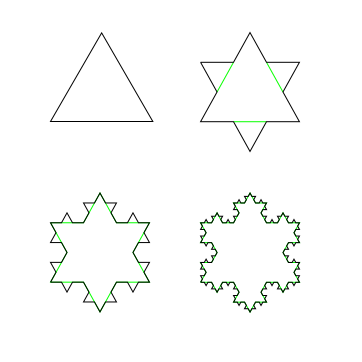
\includegraphics[width=0.3\textwidth]{KochFlake}
    \caption{The first four iterations of the Koch snowflake.}
    \label{fig:koch_snowflake}
\end{figure}

Then $K$ is homeomorphic to the circle $S^1$. For $s = \log/\log 3$, then we have $0 < \H^s(K) < \infty$ and in fact,
\begin{align*}
    \dim_{\H}(K) = \frac{\log 4}{\log 3}.
\end{align*}
\end{example}

\medskip

\begin{proposition}\label{prop_15}
In the definition of the Hausdorff measure, we can always assume that
\begin{enumerate}[label=(\alph*)]
    \item all sets $A_i$ are closed;
    
    \item or all sets $A_i$ are open.
\end{enumerate}
\end{proposition}
\begin{proof}
~\begin{enumerate}[label=(\alph*)]
    \item It is obvious, since $\operatorname{diam} \overline{A_i} = \operatorname{diam} A_i$ and we can replace $A_i$ by its closure.
    
    \item For any $E$ and fixed $\delta > 0$, there exists a family $\{A_i\}$ such that
    \begin{align*}
        \frac{\omega_s}{2^s} \sum^\infty_{i=1} (\operatorname{diam} A_i)^s \leq \H^s_{\varepsilon}(E) + \frac{\delta}{2}, \quad \operatorname{diam} A_i < \varepsilon.
    \end{align*}
    Let $U_i = \bigcup_{x \in A_i} B(x, r_i)$ such that $A_i \subset U_i$, and $U_i$ is open. Also, 
    \begin{align*}
        \operatorname{diam} U_i \leq \operatorname{diam} A_i + 2r_i < \varepsilon,
    \end{align*}
    for some $r_i$ small enough. And we can take $r_i$ small such that
    \begin{align*}
        \frac{\omega_s}{2^s} (\operatorname{diam} U_i)^s \leq \frac{\omega_s}{2^s} (\operatorname{diam} A_i)^s + \frac{\delta}{2^{i+1}}.
    \end{align*}
    
    Then, since $\{U_i\}$ is also a covering of $E$ with $\operatorname{diam} U_i < \varepsilon$, then
    \begin{align*}
        \H^s_{\varepsilon}(E) \leq \frac{\omega_s}{2^s} (\operatorname{diam} U_i)^s \leq \frac{\omega_s}{2^s} (\operatorname{diam} A_i)^s + \frac{\delta}{2} \leq \H^s_{\varepsilon}(E) + \delta,
    \end{align*}
    which implies
    \begin{align*}
        \H^s_{\varepsilon}(E) = \inf \frac{\omega_s}{2^s} (\operatorname{diam} U_i)^s,
    \end{align*}
    and the infimum is taken over all open coverings $\{U_i\}$.
\end{enumerate}
\end{proof}

\medskip

\begin{corollary}\label{coro_15}
In the definition of $\H^s$ on $\mathbb{R}$, we can take coverings by open intervals.
\end{corollary}
\begin{proof}
We can take coverings by open sets, but each open set is contained in an open interval of equal diameter.
\end{proof}

\medskip

Recall that $\H^s$ is a metric outer measure on a metric space $X$. Also, $\H^s$ restricted to $\BB(X)$ is countably additive, i.e. $\H^s$ is a Borel measure.\footnote{A {\em Borel measure} is any measure $\mu$  defined on the $\sigma$-algebra of Borel sets\cite{4}.}

\medskip

\begin{theorem}\label{theorem_119}
$\H^1$ is a measure on $\BB(\mathbb{R})$ such that
\begin{align}\label{theorem_119_1}
    \H^1((a,b)) = b - a,
\end{align}
if $- \infty < a < b < \infty$. Moreover, $\H^1$ is a unique measure with this property, that is, if $\mu$ is a measure on $\BB(\mathbb{R})$ such that $\mu((a,b)) = b - a$ if $- \infty < a < b < \infty$, then $\mu(E) = \H^1(E)$ for all $E \in \BB(\mathbb{R})$.
\end{theorem}

\medskip

$\H^1$ is a measure on $\BB(\mathbb{R})$. Assuming condition (\ref{theorem_119_1}), the uniqueness is easy to prove. 

\medskip

\begin{theorem}\label{theorem_120}
Let $X$ be a metric space, $\mu$ is a measure on $\BB(X)$, $X = \bigcup^\infty_{i=1}U_i$, where $U_i$ is open and $\mu(U_i) < \infty$. Suppose $\nu$ is another measure such that for any open set $U \subset X$, $\nu(U) = \mu(U)$, then for any $E \in \BB(X)$, $\nu(E) = \mu(E)$.
\end{theorem}
\begin{proof}
Since $X$ is a countable union of open sets with finite measure, by Theorem \ref{theorem_114}, then
\begin{align*}
    \mu(E) = \inf_{\substack{U \subset E\\ U - \text{open}}} \mu(U) = \inf_{\substack{U \subset E\\ U - \text{open}}} \nu(U) = \nu(E).
\end{align*}
\end{proof}

\medskip

Now let's use this theorem to prove the uniqueness of the previous theorem.

\medskip

\begin{proof}[Proof of Theorem \ref{theorem_119}]
~\begin{enumerate}[label=(\alph*)]
    \item Since $\H^1((a,b)) = \mu((a,b))$, by Corollary \ref{coro_15}, $\H^1(U) = \mu(U)$ for any open set $U \subset \mathbb{R}$. Thus, by Theorem \ref{theorem_120}, $\H^1(E) = \mu(E)$ for any $E \in \BB(\mathbb{R})$. Hence, the uniqueness is proved.
    
    \item It remains to prove that $\H^1((a,b)) = b - a$. 

    First, for any $\varepsilon > 0$, divide $[a,b]$ into small intervals $I_1, I_2, \cdots$, such that $\operatorname{diam} I_i < \varepsilon$. Note that $\sum^\infty_{i=1}\operatorname{diam} I_i = b - a$. Then,
    \begin{align*}
        \H^1_{\varepsilon}([a,b]) \leq \frac{\omega_1}{2^1} \sum^\infty_{i=1}(\operatorname{diam} I_i)^1 = b - a,
    \end{align*}
    since $\omega_1 = \operatorname{vol}\left(B^1(0,1)\right) = \operatorname{vol}\left((-1,1)\right) = 2$. Letting $\varepsilon \to 0$ gives $\H^1([a,b]) \leq b - a$.
    
    Second, taking infimum over coverings by open intervals $[a,b] \subset \bigcup^\infty_{i=1}U_i$, where $U_i$ is open interval and $\operatorname{diam} U_i < \varepsilon$ and then we have
    \begin{align*}
        \H^1_{\varepsilon}([a,b]) = \inf \sum^\infty_{i=1} \operatorname{diam} U_i.
    \end{align*}
    Since $[a,b]$ is compact, then there exists finite coverings of $[a,b]$ by open intervals. Choose a finite open covering $\{I_i\}$ from $\{U_i\}$ such that $[a,b] \subset \bigcup^k_{i=1} I_i$, then 
    \begin{align*}
        \sum^\infty_{i=1}\operatorname{diam} U_i \geq \sum^k_{i=1} \operatorname{diam}I_i \geq b - a.
    \end{align*}
    Taking infimum over all covering by open intervals with $\operatorname{diam}U_i < \varepsilon$ implies
    \begin{align*}
        \H^1([a,b]) = \inf \sum^\infty_{i=1} \operatorname{diam}U_i \geq b - a.
    \end{align*}
    
    It follows that $\H^1([a,b]) = b - a$, and thus $\H^1((a,b)) = b - a$.
\end{enumerate}
\end{proof}

\medskip

Let's talk more about properties of the Hausdorff measure.

\medskip

\begin{theorem}\label{theorem_121}
For $0 \leq s < \infty$ and every $E \subset X$ (not necessarily measurable), there is a sequence of open sets $V_1 \supset V_2 \supset V_3 \supset \cdots \supset E$ such that 
\begin{align*}
    E \subset \widetilde{E} \coloneqq \bigcap^\infty_{i=1} V_i,
\end{align*}
and $\H^s(E) = \H^s (\widetilde{E})$.
\end{theorem}
\begin{proof}
Note that $\widetilde{E}$ is $G_\delta$ set and hence Borel.

If $\H^s(E) = \infty$, take $v_i = X$ for all $I \in \mathbb{N}$ would yield the statement.

If $\H^s(E) < \infty$, by Proposition \ref{prop_15}, we can taking coverings by open sets in the definition of $\H^s$. So, we could find a covering $\{U_{i_j}\}$ such that
\begin{align*}
    E \subset \bigcup^\infty_{j=1} U_{i_j} \coloneqq U_i, \quad \operatorname{diam} U_{i_j} < \frac{1}{i}.
\end{align*}
and by the definition of $\H^s_{1/i} (E)$, we have
\begin{align*}
    \frac{\omega_s}{2^s} \sum^\infty_{j=1} \left(\operatorname{diam} U_{i_j}\right)^s \leq \H^s_{1/i} (E) + \frac{1}{i}.
\end{align*}

Let $V_i = \bigcap^i_{k=1}U_k$ be open, and clearly, $V_1 \supset V_2 \supset V_3 \supset \cdots \supset E$. Also, 
\begin{align*}
    \widetilde{E} \coloneqq \bigcap^\infty_{i=1} V_i = \bigcap^\infty_{i=1} U_i.
\end{align*}

We need to prove that $\H^s(E) = \H^s (\widetilde{E})$, and since $E \subset \widetilde{E}$ implies $\H^s(E) \leq \H^s(\widetilde{E})$, it remains to prove that $\H^s(E) \geq \H^s(\widetilde{E})$. Clearly,
\begin{align*}
    \widetilde{E} \subset U_i = \bigcup^\infty_{j=1} U_{i_j},
\end{align*}
then $\{U_{i_j}\}$ is a covering of $\widetilde{E}$ with $\operatorname{diam} U_{i_j} < 1/i$. Therefore,
\begin{align*}
    \H^s_{1/i}(\widetilde{E}) \leq \frac{\omega_s}{2^s} \sum^\infty_{j=1} \left(\operatorname{diam} U_{i_j}\right)^s \leq \H^s_{1/i}(E) + \frac{1}{i},
\end{align*}
and letting $i \to \infty$ gives
\begin{align*}
    \H^s(\widetilde{E}) \leq \H^s(E).
\end{align*}
Thus, $\H^s(E) = \H^s (\widetilde{E})$.
\end{proof}

\medskip

\begin{corollary}
If $0 \leq s < \infty$, $\H^s(X) < \infty$ and $E \subset X$ (not necessarily measurable), then \begin{align*}
    \H^s(E) =  \inf_{\substack{U \supset E\\ U - \text{open}}} \H^s(U).
\end{align*}
\end{corollary}
\begin{proof}
Let $V_i$ be as in the previous theorem. Clearly, $\H^1(V_1) \leq \H^s(X) < \infty$ and then, by Theorem \ref{theorem_111}(g) and Corollary \ref{coro_1111}, we have
\begin{align*}
    \lim_{i\to\infty} \H^1(V_i) = \H^s\left( \bigcap^\infty_{i=1} V_i\right) = \H^s(\widetilde{E}) = \H^s(E).
\end{align*}
\end{proof}

\medskip

\begin{remark}
Comparing this corollary with Theorem \ref{theorem_114}, we does not require $E$ being Borel set in the corollary.
\end{remark}

\medskip

\begin{theorem}
Let $E \subset X$ be any $\H^s$-measurable set, $0 \leq s < \infty$. If $\H^s(E) < \infty$, then \begin{align*}
    \H^s(E) = \sup_{\substack{C \subset E\\ C - \text{closed}}} \H^s(C).
\end{align*}
\end{theorem}
\begin{proof}
It is enough to prove that for any $\varepsilon > 0$, there exists a $F_\sigma$ subset of $E$ with $\H^s(F_\sigma) > \H^s(E) - \varepsilon$. For fixed $\varepsilon > 0$, by Theorem \ref{theorem_121}, let $\widetilde{E} = \bigcap^\infty_{i=1} V_i$, $V_i$ is open, such that $V_1 \supset V_2 \supset V_3 \supset \cdots \supset E$ and $\H^s(E) = \H^s(\widetilde{E})$. Hence, $\widetilde{E}$ is a $G_\delta$ set.

Since $E$ has finite measure, so does $\widetilde{E}$. Also, since $E \subset \widetilde{E}$, we have $\H^s(\widetilde{E} \setminus E) = 0$. 

We claim that each open set is a union of an increasing sequence of closed sets.\footnote{Let $E \subset X$ be open. Define $C_i = \left\{x \,|\, \operatorname{dist}(x, (X\setminus E)) \geq 1/i\right\}$, then $C_1 \subset C_2 \subset \cdots$, and $E = \bigcup^\infty_{i=1}C_i$. This is based on an example in $\mathbb{R}^n$: \url{https://math.stackexchange.com/a/1620262}.}Then, $V_i$ is a union of such closed sets $F_i$. Since $E \subset V_i$, then there exists a closed set $F_i \subset V_i$ such that $\H^s(E \setminus F_i) < \varepsilon / 2^i$. Define
\begin{align*}
    F \coloneqq \bigcap^\infty_{i=1} F_i \subset \bigcap^\infty_{i=1} V_i = \widetilde{E},
\end{align*}
then
\begin{align*}
    \H^s(E \setminus F) = \H^s \left(\bigcup^\infty_{i=1} (E \setminus F_i)\right) < \varepsilon.
\end{align*}
Also, $\H^s(F \setminus E) \leq \H^s(\widetilde{E} \setminus E) = 0$. Therefore, there is a $G_\delta$ set of $G$ such that $F \setminus E \subset G$ and $\H^s(G) = 0$. 

Clearly, $F \setminus G$ is $F_\sigma$ set. Indeed, $G = \bigcap^\infty_{i=1} G_i$, and since $F \setminus G_i$ is closed, then
\begin{align*}
    F \setminus G = F \setminus \left(\bigcap^\infty_{i=1} G_i\right) = \bigcup^\infty_{i=1} (F \setminus G_i)
\end{align*}
is $F_\sigma$. Also, $F \setminus G \subset E$. Indeed, for $x \in F \setminus G$, we have $x \in F, x \notin G$. Since $F \setminus E \subset G$, then $x \in E$ and hence $F \setminus G \subset E$. Since $\H^s(G) = 0$, then 
\begin{align*}
    \H^s(F \setminus G) = \H^s(F) \geq \H^s(E \cap F) = \H^s(E) - \H^s(E \setminus F) > \H^s(E) - \varepsilon,
\end{align*}
and $F \setminus G$ is the subset we seek.
\end{proof}

\medskip

\begin{remark}
Comparing this theorem with Theorem \ref{theorem_114}, we does not require $X$ being of finite measure in this theorem.
\end{remark}

\medskip

\begin{theorem}
If $0 \leq s < \infty$ and $A_1 \subset A_2 \subset \cdots$ is an increasing sequence of not necessarily measurable sets, then
\begin{align*}
    \H^s \left(\bigcup^\infty_{i=1}A_i\right) = \lim_{i\to\infty} \H^s(A_i).
\end{align*}
\end{theorem}
\begin{proof}
It suffices to show $\H^s \left(\bigcup^\infty_{i=1}A_i\right) \geq \lim_{i\to\infty} \H^s(A_i)$, since the other direction is obvious by the fact that $\lim_{i\to\infty}A_i \subset \bigcup^\infty_{i=1}A_i$.

Let $A_i \subset \widehat{A}_i$, where $\widehat{A}_i$ is a Borel set\footnote{This is possible by Theorem \ref{theorem_121} that any set (not necessarily measurable) is contained in a $G_\delta$ set of equal measure.}and $\H^s(A_i) = \H^s(\widehat{A}_i)$. Define $\widetilde{A}_i = \bigcap^\infty_{j=i} \widehat{A}_j$, and $\widetilde{A}_i$ is also Borel. Then, $A_i \subset \widetilde{A}_i$. Indeed,
\begin{align*}
    A_i \subset A_{i+1} & \subset \widehat{A}_{i+1}, \\
    A_i \subset A_{i+2} & \subset \widehat{A}_{i+2}, \\
    \vdots & 
\end{align*}
and hence $A_i \subset \bigcap^\infty_{j=i} \widehat{A}_i = \widetilde{A}_i$. Also, since $A_i \subset \widetilde{A}_i \subset \widehat{A}_i$ and $\H^s(A_i) = \H^s(\widehat{A}_i)$, then $\H^s(A_i) = \H^s(\widetilde{A}_i)$. Note that $\widetilde{A}_1 \subset \widetilde{A}_2 \subset \cdots$ are measurable sets, thus we have 
\begin{align*}
    \H^s\left(\bigcup^\infty_{i=1}A_i\right) \leq \H^s\left(\bigcup^\infty_{i=1}\widetilde{A}_i\right) = \lim_{i\to\infty} \H^s(\widetilde{A}_i) = \lim_{i\to\infty} \H^s(A_i),
\end{align*}
which is exactly the inequality we need.
\end{proof}

\medskip

\section{Lebesgue measure}

Consider a closed interval in $\mathbb{R}$,
\begin{align}\label{closed_interval}
    P = [a_1,b_1] \times \cdots [a_n,b_n] \subset \mathbb{R}^n,
\end{align}
and we define its volume as 
\begin{align*}
    \left|P\right| \coloneqq (b_1-a_1) \cdots (b_n-a_n).
\end{align*}

\medskip

\begin{definition}
For any $A \subset \mathbb{R}^n$, the outer Lebesgue measure of $A$ is defined as
\begin{align*}
    \mathcal{L}^*_n(A) = \inf \sum^\infty_{i=1} \left|P_i\right|,
\end{align*}
where the infimum is taken over all coverings 
\begin{align*}
    A \subset \bigcup^\infty_{i=1} P_i,
\end{align*}
by intervals as in (\ref{closed_interval}). $\mathcal{L}^*_n$-measurable sets are called Lebesgue measurable. $\mathcal{L}^*_n$ restricted to Lebesgue measurable sets is called Lebesgue measure and is denoted by $\mathcal{L}_n$.
\end{definition}

\medskip

\begin{theorem}
$\mathcal{L}^*_n$ is a metric outer measure.
\end{theorem}

\medskip

\begin{remark}
By Theorem \ref{theorem_113}, $\BB(\mathbb{R}^n)$ is Lebesgue measurable.
\end{remark}

\medskip

\begin{corollary}\label{coro_17}
All Borel sets in $\mathbb{R}^n$ are Lebesgue measurable. 
\end{corollary}

\medskip

\begin{remark}\label{remark_17}
Recall that if $\mu^*$ is an outer measure, by Proposition \ref{prop_14}, all sets $A$ such that $\mu^*(A) = 0$ are $\mu^*$-measurable. Therefore, if $\mathcal{L}^*_n(A) = 0$, then $A$ is Lebesgue measurable, and $\mathcal{L}_n(A) = 0$. Note that $\mathcal{L}_n(A) = 0$ if and only if for all $\varepsilon > 0$, there is a family of closed intervals $\{P_i\}$ such that 
\begin{align*}
    A \subset \bigcup^\infty_{i=1} P_i, \quad \text{and} \quad \sum^\infty_{i=1} \left|P_i\right| < \varepsilon.
\end{align*}
\end{remark}

\medskip

\begin{theorem}\label{theorem_125}
If $P$ is a closed interval as in (\ref{closed_interval}), then $\mathcal{L}_n(P) = \left|P\right|$.
\end{theorem}

We often write $\left|A\right|$ to denote the Lebesgue measure of a Lebesgue measurable set $A$.

\begin{proof}
By definition,
\begin{align*}
    \mathcal{L}_n(P) = \inf \sum^\infty_{i=1} \left|P_i\right|, \quad P \subset \bigcup^\infty_{i=1} P_i.
\end{align*}
Taking covering of $P$ by itself, then $P \subset P$, then $\mathcal{L}_n(P) \leq \left|P\right|$.

It remains to show that $\left|P\right| \leq \sum^\infty_{i=1} \left|P_i\right|$. And we need a lemma to prove this.

\begin{lemma}\label{lemma_121}
If $P \subset \bigcup^k_{i=1} P_i$ is a finite covering of a closed interval $P$ by closed intervals $P_i$, then $\left|P\right| \leq \sum^k_{i=1} \left|P_i\right|$.
\end{lemma}
\begin{proof}[``Proof'']
We use the Riemann integral to prove this. Since $P \subset \bigcup^k_{i=1} P_i$, then
\begin{align*}
    \chi_P \leq \sum^k_{i=1} \chi_{P_i}.
\end{align*}
Then, we have
\begin{align*}
    \left|P\right| = \int_{\mathbb{R}^n} \chi_P \leq \sum^k_{i=1} \int_{\mathbb{R}^n} \chi_{P_i} = \sum^k_{i=1} \left|P_i\right|.
\end{align*}
\end{proof}
\begin{figure}[H]
    \centering
    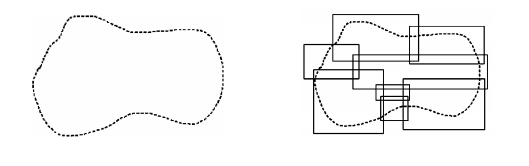
\includegraphics[width=0.6\textwidth]{closed_interval_covering.png}
    \caption{Example of a set covered by intervals(From \cite{6}).}
    \label{fig:closed_intervals}
\end{figure}

Now we can complete the proof of the theorem. Each interval $P_i$ is contained in a slightly bigger open interval $P_i^\varepsilon$ such that
\begin{align*}
    \left|\overline{P_i^\varepsilon}\right| = \left|P_i\right| + \frac{\varepsilon}{2^i},
\end{align*}
where $\overline{P_i^\varepsilon}$ is the closure of $P_i^\varepsilon$. Since $P$ is compact, then we can select a finite subcovering 
\begin{align*}
    P \subset \bigcup^k_{j=1} P_{i_j}^\varepsilon,
\end{align*}
and the lemma implies
\begin{align*}
    \left|P\right| \leq \sum^k_{j=1} \left|\overline{P_{i_j}^\varepsilon} \right| \leq \sum^\infty_{j=1} \left| \overline{P_{i}^\varepsilon} \right| = \sum^\infty_{i=1} \left|P_{i}\right| + \varepsilon,
\end{align*}
since $\varepsilon > 0$ is arbitraty, then the theorem follows.
\end{proof}

\medskip

\begin{proposition}
Let $P$ ba an open interval.
\begin{enumerate}
    \item[(a)] If $P = (a_1,b_1) \times \cdots (a_n,b_n)$ is a bounded interval, then 
    \begin{align*}
        \mathcal{L}_n(P) = (b_1-a_1) \cdots (b_n-a_n).
    \end{align*}
    
    \item[(b)] $\mathcal{L}_n(\partial P) = 0$.
    
    \item[(c)] If $P$ is an unbounded interval in $\mathbb{R}_n$ and has nonempty interior (i.e. each side has positive length and at least one of the sides has infinite length, which is of form $(-\infty,b), (a,\infty)$ or $(-\infty,\infty)$), then $\mathcal{L}_n(P) = \infty$.
\end{enumerate}
\end{proposition}
\begin{proof}
~\begin{enumerate}
    \item[(a)] For $P$, we could find a slightly smaller interval $P_\varepsilon$ contained in $P$ and a slightly bigger interval $P^\varepsilon$ which contains $P$, where\footnote{Here, $\bigtimes$ denotes the Cartesian product.}
    \begin{align*}
        P_\varepsilon = \bigtimes^n_{i=1} \left[a_i+\varepsilon,b_i-\varepsilon\right], \quad P^\varepsilon = \bigtimes^n_{i=1} \left[a_i-\varepsilon,b_i+\varepsilon\right].
    \end{align*}
    Then, $\mathcal{L}_n(P_\varepsilon) \leq \mathcal{L}_n(P) \leq \mathcal{L}_n(P^\varepsilon)$. Letting $\varepsilon \to 0$ yields the result:
    \begin{align*}
        (b_1-a_1) \cdots (b_n-a_n) \leftarrow \mathcal{L}_n(P_\varepsilon) \leq \mathcal{L}_n(P) \leq \mathcal{L}_n(P^\varepsilon) \to (b_1-a_1) \cdots (b_n-a_n).
    \end{align*}
    
    \item[(b)] $\mathcal{L}_n(\partial P) =  \mathcal{L}_n(\overline{P}) - \mathcal{L}_n(\operatorname{int}(P)) = 0$.
    
    \item[(c)] $P$ contains closed intervals of arbitrarily large measure.
\end{enumerate}
\end{proof}

\medskip

\begin{corollary}\label{coro_19161}
If $k < n$, then $\mathcal{L}_n (\mathbb{R}^k) = 0$.
\end{corollary}
\begin{proof}
It suffice to show that $[-k,k]^{k} \times \{0\}^{n-k}$ has Lebesgue measure zero for all $k \in \mathbb{N}$.\footnote{It is based on the proof of  $\mathbb{R}^n\times\{0\}$ has measure zero in $\mathbb{R}^{n+1}$: \url{https://math.stackexchange.com/a/524155}.} 

For any $\varepsilon > 0$, choose $\delta > 0$ such that
\begin{align*}
    (2\delta)^{n-k} (2k+2\varepsilon)^k < \varepsilon.
\end{align*}
Now we define $$U_k = (-k-\varepsilon,k+\varepsilon)^k \times (-\delta,\delta)^{n-k},$$ 
and clearly $U_k$ contains $[-k,k]^{k} \times \{0\}^{n-k}$. Also, by the choice of $\delta$, $\mathcal{L}_n(U_k) < \varepsilon$, and since
\begin{align*}
    \mathcal{L}_n(\mathbb{R}^k) = \lim_{k\to\infty} \mathcal{L}_n\left([-k,k]^{k} \times \{0\}^{n-k}\right) < \varepsilon,
\end{align*}
we have $\mathcal{L}_n(\mathbb{R}^k) = 0$.
\end{proof}

\medskip

\begin{proof}[Second Proof of Corollary \ref{coro_19161}]
Finite intervals in $\mathbb{R}^k$ are contained in $\partial P$ for some interval $P$ in $\mathbb{R}^n$. Then, finite intervals in $\mathbb{R}^k$ have Lebesgue measure zero. Since $\mathbb{R}^k$ is a union of finite intervals in $\mathbb{R}^k$, then $\mathcal{L}_n(\mathbb{R}_k) = 0$.
\end{proof}

\medskip

\begin{theorem}\label{theorem_122}
For an arbitrary set $E \subset \mathbb{R}^n$ (not necessarily measurable),
\begin{align*}
    \mathcal{L}_n^*(E) = \inf_{\substack{U \subset E\\ U - \text{open}}} \mathcal{L}_n(U).
\end{align*}
\end{theorem}
\begin{proof}
Clearly, $\mathcal{L}_n^*(E) \leq \inf_{U \subset E} \mathcal{L}_n(U)$. It remains to show the other direction.

By definition, $\mathcal{L}^*_n(E) = \inf \sum^\infty_{i=1} \left|P_i\right|$, $E \subset \bigcup_i P_i$, where $P_i$ are closed intervals. Now let $P_i^\varepsilon$ be open interval such that $P_i \subset P_i^\varepsilon$ and
\begin{align*}
    \left|P_i^\varepsilon\right| = \left|P_i\right| + \frac{\varepsilon}{2^i}.
\end{align*}

This approximation yields
\begin{align*}
    \mathcal{L}_n^*(E) = \inf \sum^\infty_{i=1} \left|P_i\right|, \quad E \subset \bigcup^\infty_{i=1} P_i,
\end{align*}
where $P_i$ are open. Indeed, by the subadditivity of the outer measure, $\mathcal{L}_n^*(E) \leq \sum^\infty_{i=1} \left|P_i\right|$, which implies $\mathcal{L}_n^*(E) \leq \inf \sum^\infty_{i=1} \left|P_i\right|$. Also, every closed interval can be approximated by a slighter bigger open interval, and this implies the equality.

Now, for $E \subset \bigcup^\infty_{i=1}P_i$, $P_i$ are open intervals, by Theorem \ref{theorem_125},
\begin{align*}
    \sum^\infty_{i=1} \left|P_i\right| \geq \left|\bigcup^\infty_{i=1}P_i\right| = \mathcal{L}_n\left(\bigcup^\infty_{i=1}P_i\right) \geq \inf_{U \supset E} \mathcal{L}_n(U),
\end{align*}
where $U$ is open, and taking the infimum over all coverings $E \subset \bigcup^\infty_{i=1}P_i$ by open intervals yields
\begin{align*}
    \mathcal{L}_n^*(E) \geq  \inf_{U \supset E} \mathcal{L}_n(U).
\end{align*}
\end{proof}

\medskip

So how to compute $\mathcal{L}_n(U)$ for open set $U$? Let's introduce the dyadic cubes. Consider cubes vertices in $\mathbb{Z}^n$, and divide each cubes into $2^k$ cubes, $k = 0,1,2,\cdots$. 

\medskip

\begin{theorem}\label{theorem_123}
An arbitrary open set in $\mathbb{R}^n$ is a union of closed dyadic cubes with pairwise disjoint interiors. Then the Lebesgue measure of the open set equals the sum of the measures of these cubes.
\end{theorem}
\begin{figure}[H]
    \centering
    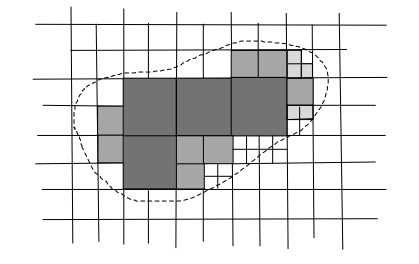
\includegraphics[width=0.5\textwidth]{dyadic_cube.png}
    \caption{Example of open set represented by the dyadic cubes in $\mathbb{R}^2$(From \cite{6}).}
    \label{fig:dyadic_cube}
\end{figure}

\medskip

Recall that by a $G_\delta$ set we mean a set of the form $G = \bigcap^\infty_{i=1} G_i$, where $G_i \subset X$ are open and by a $F_\sigma$ set we mean a set of the form $F = \bigcap^\infty_{i=1} F_i$, where $F_i \subset X$ are closed. Clearly, all $G_\delta$ and $F_\sigma$ sets are Borel sets.

\medskip

\begin{theorem}\label{theorem_124}
Let $A \subset \mathbb{R}^n$, then the following conditions are equivalent:
\begin{enumerate}[label=(\alph*)]
    \item $A$ is Lebesgue measurable;
    
    \item For every $\varepsilon > 0$, there is an open set $G$ such that $A \subset G$ and $\L^*_n(G\setminus A) < \varepsilon$;
    
    \item There is a $G_\delta$ set $H$ such that $A \subset H$ and $\L^*_n(H\setminus A) = 0$;
    
    \item For every $\varepsilon > 0$, there is a closed set $F$ such that $F \subset A$ and $\L^*_n(A\setminus F) < \varepsilon$;
    
    \item There is a $F_\sigma$ set $M$ such that $M \subset A$ and $\L^*_n(A\setminus M) = 0$;
    
    \item For every $\varepsilon > 0$, there is an open set $G$ and a closed set $F$ such that $F \subset A \subset G$ and $\L_n(G \setminus F) < \varepsilon$.
\end{enumerate}
\end{theorem}
\begin{proof}
~\begin{enumerate}
    \item[(a)]$\Rightarrow$ (b) Every measurable set can be represented as a union of sets with finite measure $A = \bigcup^\infty_{i=1}A_i$, $\L_n(A_i) < \infty$, where $A_i$ is Lebesgue measurable and $\L_n(A_i) < \infty$. Indeed, since $A$ is arbitrary Lebesgue measurable set, then we can define $A_i = A \cap B(0,i), i = 1,2,\cdots,n$, where $B(0,i) \subset \mathbb{R}^n$ is the closed ball centered at the origin with radius $i$. Since $A$ is measurable and bounded, then $\L_n(A_i) < \infty$. By Theorem \ref{theorem_122}, for every $i$, there is an open set $G_i$ such that $A_i \subset G_i$ and $\L_n(G_i\setminus A_i) < \varepsilon / 2^i$. Hence $A \subset \bigcup^\infty_{i=1} G_i \coloneqq G$, and $\L_n(G \setminus A) \leq \sum^\infty_{i=1} \L_n(G_i \setminus A_i) = \varepsilon$.\footnote{Indeed, since $(G \setminus A) \subset (G \setminus A_i)$, then $G \setminus A = \bigcup^\infty_{i=1} (G_i \setminus A) \subset \bigcup^\infty_{i=1} (G_i \setminus A_i).$}
    
    \item[(b)]$\Rightarrow$ (c) By (b), we can find an open set $G_i$ such that $A \subset G_i$ and $\L_n^*(G_i\setminus A) < 1/i$. Let $H = \bigcap^\infty_{i=1} G_i$, then $H$ is $G_\delta$ set and $A \subset H$. Then, $\L_n^*(H\setminus A) \leq 1/i$ for every $i \in \mathbb{N}$, which yields $\L_n^*(H\setminus A) = 0$. Hence, by Remark \ref{remark_17}, $\L_n(H \setminus A) = 0$.
    
    \item[(c)]$\Rightarrow$ (a) We know that $A = H \setminus (H \setminus A)$, $H$ is $G_\delta$ set and it follows from Corollary \ref{coro_17}, $H$ is measurable. Since $H \setminus A$ is measurable, hence $A$ is also measurable.
    
    \item[(a)] $\Leftrightarrow	$ (d) $\Leftrightarrow$ (e)\footnote{It follows from the equivalence of the conditions (a), (b) and (c) applied to the set $\mathbb{R}^n\setminus A$.} $A$ is measurable, then $\mathbb{R}^n \setminus A$ is also measurable. By (b), there is an open set $G$ such that $(\mathbb{R}^n \setminus A) \subset G$ and $\L_n^*(G \setminus (\mathbb{R}^n \setminus A)) < \varepsilon$. Let $F \coloneqq \mathbb{R}^n \setminus G \subset A$, then $F$ is closed. Since $A \setminus F = G \setminus (\mathbb{R}^n \setminus A)$, then $\L_n(A \setminus F) < \varepsilon$, which indicates (d).
    
    Now for $\mathbb{R}^n \setminus A$, by (c), there exists a $G_\delta$ set $H$ such that $(\mathbb{R}^n \setminus A) \subset H$ and $\L_n^*(H \setminus (\mathbb{R}^n \setminus A)) = 0$. Let $M \coloneqq \mathbb{R}^n \setminus H \subset A$, then $M$ is a $F_\sigma$ set. Since $A \setminus M = H \setminus (\mathbb{R}^n \setminus A$, then $\L_n(A \setminus M) = 0$, which indicates (e).
    
    \item[(a)] $\Rightarrow$ (f) By (d), there is a closed set $F \subset A$ such that $\L_n(A \setminus F) < \varepsilon/2$. By (b), there is an open set $G \supset A$ such that  $\L_n(G \setminus A) < \varepsilon/2$. Hence, $F \subset A \subset G$ and $\L_n(G \subset F) < \varepsilon/2 + \varepsilon/2 = \varepsilon$.
    
    \item[(f)] $\Rightarrow$ (a) There exists a closed set $F_i$ and an open set $G_i$ such that $\L_n(G_i\setminus F_i) < 1/i$. Let $H \coloneqq \bigcap^\infty_{i=1} G_i$, then $H$ is a $G_\delta$ set and $A \subset H$. Then,
    \begin{align*}
        \L_n^*(H \setminus A) \leq \L_n^*\left(H \setminus \bigcup^\infty_{i=1}F_i\right) \leq \L_n^*\left(\bigcap^\infty_{i=1}(G_i \setminus F_i)\right) = 0.
    \end{align*}
    Therefore, (f) implies (c), and hence (a).\footnote{The second inequality follows from that if $x \in H \setminus \bigcup^\infty_{i=1}F_i$, then $x \in G_i$ but $x \notin F_i$ for all $i$. Hence, $x \notin G_i \setminus F_i$ for all $i$, which is equivalent to $x \in \bigcap^\infty_{i=1} (G_i \setminus F_i)$.}
\end{enumerate}
\end{proof}

\medskip

The Lebesgue measure has an important property of being invariant under translations, i.e. $E \subset \mathbb{R}^n$ is Lebesgue measurable if and only if for all $a \in \mathbb{R}^n$, $E+a = \{x+a\,|\, x \in E\}$ is Lebesgue measurable. Moreover, $\L_n(E) = \L_n(A)$. Now we want to discuss an example of set that is not Lebesgue measurable.

\medskip

\begin{theorem}[\bf Vitali]
There is a set $E \in \mathbb{R}^n$ which is not Lebesgue measurable.
\end{theorem}
\begin{proof}[``Idea'']
We will prove the theorem for $n = 1$, and the same argument can be applied to an arbitrary $n$. The idea is to find a countable family of pairwise disjoint and isometric sets $V_i$ whose union $E$ contains $(0,1)$ and is contained in $(-1,2)$, that is find countable many $V_i \in (-1,2)$ such that $V_i \cap V_j = \emptyset$ for all $i \neq j$, and for all $i$, there is a set $V \in (0,1)$ such that $V_i$ is a translation of $V$. Also, $(0,1) \subset \bigcup^\infty_{i=1} V_i \subset (-1,2)$. Then $V$ cannot be Lebesgue measurable.

Suppose $V$ is Lebesgue measurable. Since $V_i$ is a translation of $V$, then $\L_1(V) = \L_1(V_i)$ for all $i$. If $\L_1(V) = 0$, then
\begin{align*}
    \L_1((0,1)) \leq \sum^\infty_{i=1} \L_1(V_i) = 0,
\end{align*}
which is a contradiction.

If $\L_1(V) > 0$, then
\begin{align*}
    3 = \L_1((-1,2)) \geq \L_1\left(\bigcup^\infty_{i=1} V_i\right) = \sum^\infty_{i=1} \L_1(V_i) = \infty,
\end{align*}
which is also a contradiction. Thus, $V$ is not Lebesgue measurable.
\end{proof}

\medskip

Now let's construct such $V$ properly.

\medskip

\begin{proof}[Proof of Vitali Theorem]
Consider the following equivalence relation among point in $(0,1)$, $x \sim y$ if $x - y \in \mathbb{Q}$. Therefore, $(0,1)$ is the union of a family $\mathcal{F}$ of pairwise disjoint equivalent classes 
\begin{align*}
    \{x\} = \{y \in (0,1)\,|\, x - y \in \mathbb{Q}\}.
\end{align*}
Then $\{x\} = \{y\}$ if and only if $x \sim y$. Also, $\mathbb{F} = \{\{x\}\,|\, x \in (0,1)\}$, then 
\begin{align*}
    (0,1) = \bigcup_{\{x\} \in \mathcal{F}} \{x\}.
\end{align*}
By the axiom of choice,\footnote{The construction of $V$ involves the axiom of choice, see Theorem \ref{axiom_of_choice}.} there is a set $V \subset (0,1)$ such that $V$ contains exactly one element from each equivalence class. Then, $V$ has following properties:
\begin{enumerate}[label=(\alph*)]
    \item If $x,y \in V, x \neq y$, then $x - y \notin \mathbb{Q}$. Otherwise, $\{x\} = \{y\}$.
    
    \item If $x \in (0,1)$, then there is $a \in \mathbb{Q}$ such that $x - a \in V$. Indeed, there is $y \in \{x\}$ such that $y \in V$, then $x \sim y$, which implies $y = x - a$, $a \in \mathbb{Q}$.\label{vitali_property_b}
\end{enumerate}

Next we will prove that $V$ is not Lebesgue measurable. Let
\begin{align*}
    E = \bigcup_{a\in\mathbb{Q}\cap(-1,1)} V_a,
\end{align*}
where $V_a = V + a = \{x+a\,|\, x\in V\}$. Clearly,
\begin{enumerate}[label=(\roman*)]
    \item $V_a \cap V_b = \emptyset$, if $a,b \in \mathbb{Q}, a \neq b$. Indeed, suppose $x \in (V_a \cap V_b)$, then $x = x_1 + a$ and $x = x_2 + b$, then $x_1 - x_2 = b - a \in \mathbb{Q}$. Therefore, $\{x_1\} = \{x_2\}, x_1 \neq x_2$. Hence, $x_1, x_2 \in V$ are two different points from the same equivalence class, which is a contradiction.
    
    \item $(0,1) \subset E \subset (-1,2)$. Clearly, $V \subset (0,1)$, $a \in (-1,1)$, then $V_a \subset (-1,2)$ for all $a \in \mathbb{Q}\cap(-1,1)$. Therefore, $E \subset (-1,2)$. Now let $x \in (0,1)$, then there is $y \in \mathbb{Q}$ such that $x - y \in V \subset (0,1)$ by property \ref{vitali_property_b} above. And since $x - y \in (0,1)$, then $y \in \mathbb{Q} \cap (-1,1)$, which implies $x \in V_y \subset E$. Hence, $(0,1) \subset E$.
\end{enumerate}
Now suppose $V$ is Lebesgue measurable, then each $V_a$ is measurable and since $V_a$ is a translation of $V$, then $\L_1(V) = \L_1(V_a)$. If $\L_1(V) > 0$, then $\L_1(E) = \infty$, which is a contradiction. If $\L_1(V) = 0$, then $\L_1(E) = 0$, which is also a contradiction. Thus, $V$ is not Lebesgue measurable.
\end{proof}

\medskip

The Lebesgue measure is translation invariant and $\L_n([0,1]^n) = 1$, and this two properties uniquely determine Lebesgue measure. This indicates that the
Lebesgue measure is in a sense the only natural way of measuring length, area, volume of general sets in finite-dimensional Euclidean spaces, which gives the following theorem.

\medskip

\begin{theorem}\label{theorem_126}
If $\mu$ is a measure on $\BB(\mathbb{R}^n)$ such that $\mu(a+E) = \mu(E)$ for all $a \in \mathbb{R}^n$ and $E \subset \BB(\mathbb{R}^n)$ and $\mu([0,1]^n) = 1$, then $\mu(E) = \L_n(E)$ on $\BB(\mathbb{R}^n)$.
\end{theorem}
\begin{proof}
By Corollary \ref{coro_191}, it suffice to prove that $\mu(U) = \L_n(U)$ for all open set $U$. 

Let $K$ be a face of the boundary $\partial Q$ of a unit cube $Q = [0,1]^n$, and there are $2^n$ faces. There are infinitely many pairwise parallel copies of $K$ inside $Q$, denoted by $K_1, K_2, \cdots$, shown in the following
\begin{figure}[H]
    \centering
    \begin{tikzpicture}[scale=2.5]
        \draw[-] (0,0)--(1,0)node[pos=.5,below]{$Q$};
        \draw[-] (1,0)--(1,1);
        \draw[-] (1,1)--(0,1);
        \draw[-] (0,1)--(0,0);
        \draw[-] (0,1)--(0.424,1.424);
        \draw[-] (0.424,1.424)--(1.424,1.424);
        \draw[-] (1.424,0.424)--(1.424,1.424);
        \draw[dotted,-] (0,0)--(0.424,0.424);
        \draw[dotted,-] (0.424,0.424)--(1.424,0.424);
        \draw[dotted,-] (0.424,0.424)--(0.424,1.424);
        \draw[fill=gray] (1,0)--(1,1)--(1.424,1.424)--(1.424,0.424);
        \filldraw[black] (1.106,0.7) circle (0pt) node[anchor=west]{$K$};
        \draw[-] (1,0)--(1.424,0.424);
        \draw[-] (1,1)--(1.424,1.424);
        
        \draw[-] (0.5,0)--(0.5,1);
        \draw[-] (0.5,1)--(0.912,1.424);
        \draw[dotted,-] (0.912,1.424)--(0.912,0.424);
        \draw[dotted,-] (0.912,0.424)--(0.5,0);
        \filldraw[black] (0.606,0.7) circle (0pt) node[anchor=west]{$K_1$};
    \end{tikzpicture}
    \caption{Parallel copy $K_1$ of face $K$ inside a $3$-dimensional unit cube.}
    \label{fig:unit_cube_cut}
\end{figure}
Since $\mu$ is translation invariant, then 
\begin{align*}
    \mu(K_1) = \mu(K_2) = \cdots = \mu(K).
\end{align*}
Since $\mu(Q) = 1$, then $\mu(K) = 0$. Indeed, otherwise $\mu(K) > 0$, then $1 = \mu(Q) \geq \mu\left(\bigcup_i K_i\right) = \sum_i \mu(K_i) = \infty$, which is a contradiction. This implies that $\mu(\partial Q) = 0$. 

Let $k \in \mathbb{N}$, $k > 0$ and let $Q_k = (0,2^{-k})^n$, then $\mu(\partial Q_k) = 0$. Note there are $2^{kn}$ open cubes contained in $Q$, denoted by $A_1, A_2, \cdots, A_{2^{kn}}$,\footnote{These are the dyadic cubes.} each being a translation of $Q_k$. Then, 
\begin{align*}
    2^{kn} \mu(Q_k) = \sum^{2^{kn}}_{i=1} \mu(A_i) \leq \mu(Q) = 1,
\end{align*}
which implies $\mu(Q_k) \leq 2^{-kn}$. Since $\mu(\partial Q_k) = 0$, then 
\begin{align*}
    \mu(\overline{Q}_k) = \mu(Q_k) \leq 2^{-kn}.
\end{align*}

On the other hand, $Q$ can be covered by $2^{kn}$ cubes $\overline{A}_1, \overline{A}_2, \cdots, \overline{A}_{2^{kn}}$, then
\begin{align*}
    1 = \mu(Q) \leq \sum^{2^{kn}}_{i=1} \mu(\overline{A}_i) = 2^{kn} \mu(\overline{Q}_k).
\end{align*}
Hence, $\mu(\overline{Q}_k) = \mu(Q_k) = 2^{-kn}$. Also, since $\L_n(\overline{Q}_k) = 2^{-kn}$, we have $\mu(\overline{Q}_k) = \L_n(\overline{Q}_k)$. Therefore, $\L_n = \mu$ on the dyadic cubes. 

For any open set $U \subset \mathbb{R}^n$, by Theorem \ref{theorem_123}, then $U$ can be written as a union of the dyadic cubes, that is 
\begin{align*}
    U = \bigcup^\infty_{i=1} \overline{D}_i = \left(\bigcup^\infty_{i=1} D_i\right) \cup \left(\bigcup^\infty_{i=1} \partial D_i\right),
\end{align*}
and since $\L_n(\bigcup_i \partial D_i) = \mu(\bigcup_i \partial D_i) = 0$, then 
\begin{align*}
    \mu(U) = \mu\left(\bigcup^\infty_{i=1} D_i\right) = \sum^\infty_{i=1} \mu(D_i) = \sum^\infty_{i=1} \L_n(D_i) = \L_n\left(\bigcup^\infty_{i=1} D_i\right) = \L_n(U),
\end{align*}
and thus the theorem follows.
\end{proof}

\medskip

Observe that by Corollary \ref{coro_1111}, $\H^n$ is a measure on $\BB(\mathbb{R}^n)$, and $\H^n(a+E) = \H^n(E)$ and $\H^n([0,1]^n) < \infty$. If we can prove $\H^n([0,1]^n) = 1$, then $\H^n = \L_n$ on $\BB(\mathbb{R}^n)$.

\medskip

\begin{theorem}
$\H^n = \L_n$ on $\BB(\mathbb{R}^n)$.
\end{theorem}

\medskip

Before proving this theorem, we need some propositions. Recall that $E \subset \mathbb{R}^n$ has measure zero if and only if for any $\varepsilon > 0$, there is a covering $E \subset \bigcup_i P_i$ such that $\sum_i \left|P_i\right| < \varepsilon$.

\medskip

\begin{proposition}
$E \subset \mathbb{R}^n$ has measure zero if and only if for any $\varepsilon > 0$, there is a family of balls $\{B(x_i,r_i)\}^\infty_{i=1}$ such that
\begin{align*}
    E \subset \bigcup^\infty_{i=1} B(x_i,r_i), \quad \sum^\infty_{i=1} r_i^n < \varepsilon.
\end{align*}
\end{proposition}
\begin{proof}
~\begin{enumerate}
    \item[($\Leftarrow$)] Each ball $B(x_i,r_i)$ is contained in a cube $Q_i$ of sidelength $2r_i$ so we can cover $E$ by cubes $E \subset \bigcup_i Q_i$ such that
    \begin{align*}
        \sum^\infty_{i=1} \left|Q_i\right| = \sum^\infty_{i=1} (2r_i)^n < 2^n \varepsilon,
    \end{align*}
    letting $\varepsilon \to 0$ proves this direction.
    
    \item[($\Rightarrow$)] Since $\L_n(E) = 0$, then there is an open set $U$ such that $E \subset U$, $\L_n(U) < 2^{-n}n^{-n/2} \varepsilon$. Also, by Theorem \ref{theorem_123}, $U$ is a union of the closed dyadic cubes $\overline{D}_i$ with disjoint interiors $D_i$, that is $U = \bigcup^\infty_{i=1} \overline{D}_i$. Any cube $\overline{D}$ of sidelength $\ell$ is contained in a ball of radius $r = 2\sqrt{n}\ell$,\footnote{See: \url{https://math.stackexchange.com/a/1603122}.}and $r^n = 2^nn^{n/2}|\overline{D}|$. 
    
    Therefore, $\overline{D}_i \subset B(x_i,r_i)$ of radius $r_i$ similar to the above. Thus, $U \subset \bigcup^\infty_{i=1} B(x_i,r_i)$, and
    \begin{align*}
        \sum^\infty_{i=1} r_i^n = 2^nn^{n/2} \sum^\infty_{i=1} |\overline{D}|\, = 2^nn^{n/2} \L_n(U) < \varepsilon.
    \end{align*}
\end{enumerate}
\end{proof}

\medskip

\begin{definition}
A function between metric spaces $f:(X,d_X) \to (Y,d_Y)$ is Lipschitz continuous if there is a constant $L > 0$ such that for all $x, y\in X$, $d_Y(f(x),f(y)) \leq L d_X(x,y)$.
\end{definition}

\medskip

\begin{proposition}\label{proposition_19}
If $f:\mathbb{R}^n \to \mathbb{R}^n$ is Lipschitz and $E \subset \mathbb{R}^n$ has measure zero, then $f(E)$ has measure zero.
\end{proposition}
\begin{proof}
Since $\L_n(E) = 0$, then there is a covering $E \subset \bigcup^\infty_{i=1} B(x_i,r_i)$ by balls such that $\sum^\infty_{i=1} r_i^n < L^{-n} \varepsilon$. Then, by Lipschitz continuity, we have
\begin{align*}
    f(E) \subset \bigcup^\infty_{i=1} f(B(x_i,r_i)) \subset \bigcup^\infty_{i=1} B(f(x_i),Lr_i), \quad \sum^\infty_{i=1} (Lr_i)^n < \varepsilon.
\end{align*}
Therefore, $f(E)$ can be covered by balls of radius $\rho_i = Lr_i$, $\sum^\infty_{i=1} \rho_i^n < \varepsilon$. Thus, $\L_n(f(E)) = 0$.
\end{proof}

\medskip

\begin{proposition}\label{proposition_110}
If $f:\mathbb{R}^n \to \mathbb{R}^n$ is a homeomorphism, then $A \subset \mathbb{R}^n$ is Borel set if and only if $f(A)$ is a Borel set.
\end{proposition}
\begin{proof}\footnote{This proof is based on the result in: \url{https://math.stackexchange.com/a/2833250}.}
Let $\mathfrak{B}(\mathbb{R}^n)$ be the $\sigma$-algebra generated by the family of all open sets in $\mathbb{R}^n$. Now define $\widetilde{\mathfrak{B}} = \{f(E)\,|\,E \in \mathfrak{B}(\mathbb{R}^n)\}$. Note that $\widetilde{\mathfrak{B}}$ is also a $\sigma$-algebra. Indeed, since $f$ is honeomorphism,
\begin{enumerate}[label=(\alph*)]
    \item $f(\mathbb{R}^n) = \mathbb{R}^n$, and hence $\mathbb{R}^n \in \widetilde{\mathfrak{B}}$.
        
    \item For any $f(E) \in \widetilde{\mathfrak{B}}$, we have $\mathbb{R}^n \setminus f(E) = f(\mathbb{R}^n) \setminus f(E) = f(\mathbb{R}^n \setminus E) \in \widetilde{\mathfrak{B}}$, since $\mathbb{R}^n \setminus E \in \mathfrak{B}(\mathbb{R}^n)$.
        
    \item For any $f(E_i) \in \widetilde{\mathfrak{B}}$, then $\bigcup^\infty_{i=1} f(E_i) = f \left( \bigcup^\infty_{i=1} E_i\right) \in \widetilde{\mathfrak{B}}$, since $\bigcup^\infty_{i=1} E_i \subset \BB(\mathbb{R}^n)$.
\end{enumerate}

We claim that $\widetilde{\mathfrak{B}}$ contains all open sets. Indeed, if an open set $U \in \mathbb{R}^n$, then $f^{-1}(U) \in \mathbb{R}^n$ is also open by the continuity of $f^{-1}$. Hence, $U = f\left(f^{-1}(U)\right) \in \widetilde{\mathfrak{B}}$, which implies $\mathfrak{B}(\mathbb{R}^n) \subset \widetilde{\mathfrak{B}}$. Therefore, if $A \in \mathfrak{B}(\mathbb{R}^n)$, then $f(A) \in \mathfrak{B}(\mathbb{R}^n) \subset \widetilde{\mathfrak{B}}$, and thus $f(A)$ is Borel.

Also, for any $V \in \widetilde{\mathfrak{B}}$, there exists an open set $U \in \mathfrak{B}(\mathbb{R}^n) \subset \widetilde{\mathfrak{B}}$ such that $V = f(U)$. By continuity of $f^{-1}$, $U = f^{-1}(f(U)) = f^{-1}(V)$, which implies $V \in \mathfrak{B}(\mathbb{R}^n)$, and hence $\widetilde{\mathfrak{B}} \subset \mathfrak{B}(\mathbb{R}^n)$. Thus, if $f(A)$ is Borel, then $A$ is also Borel.
\end{proof}

\medskip

\begin{remark}
It may happen for a homeomorphism $f:\mathbb{R}^n \to \mathbb{R}^n$ that $A \subset \mathbb{R}^n$ is Lebesgue measurable, but $f(A)$ is not.
\end{remark}

\medskip

As we know, $\L_n([0,1]^n) = 1$, now $Q$ is a rotation of the unit cube $[0,1]^n$, i.e. $Q = L([0,1]^n)$, where $L$ is a rotation. Then how do we know that $\L_n(Q) = 1$? This is absolutely not trivial. To show this, we need the following theorem.

\medskip

\begin{theorem}
If $L:\mathbb{R}^n\to\mathbb{R}^n$ is a non-degenerate, linear transformation represented by a matrix $A$ ($\det A \neq 0$), then $L(E)$ is Borel (Lebesgue measurable) set if and only if $E$ is Borel (Lebesgue measurable) set. Moreover,
\begin{align*}
    \L_n(L(E)) = \left|\det A\right| \L_n(E).
\end{align*}
\end{theorem}
\begin{proof}
Since $L$ is a homeomorphism, by Proposition \ref{proposition_110}, $E$ is Borel if and only is $L(E)$ is Borel. Also, by continuity, $L$ and $L^{-1}$ are Lipschitz continuous. Moreover, by Proposition \ref{proposition_19}, $\L_n(E) = 0$ implies that $\L_n(L(E)) = 0$ and if $\L_n(L(E)) = 0$, the $\L_n(E) = \L_n(L^{-1}(L(E))) = 0$. Therefore, $E$ has measure zero if and only if $L(E)$ has measure zero, that is $L$ preserves the class of sets of measure zero.

By Theorem \ref{theorem_124}(e), $E$ is Lebesgue measurable if and only if $E$ can be written as a disjoint union of a Borel set $F$ and a set $K$ of measure zero. Then, $L(E) = L(F) + L(K)$ and $L(F)$ is Borel, hence $L(E)$ is Lebesgue measurable. Therefore, $L$ preserves the class of Lebesgue measurable sets.

It remains to prove that $\L_n(L(E)) = \left|\det A\right| \L_n(E)$. Define a new measure $\mu$ on $\BB(\mathbb{R}^n)$ such that $\mu(E)= \L_n(L(E))$. Clearly, $\mu$ is translation invariant by the continuity of $L$. Let $a = \mu([0,1]^n) = \L_n(L([0,1]^n))$, then $a > 0$ because $L([0,1]^n)$ has nonempty interior. Consider the measure $E \mapsto a^{-1} \mu(E)$, then this map is translation invariant and $a^{-1} \mu([0,1]^n) = 1$. By Theorem \ref{theorem_126}, $a^{-1} \mu(E) = \L_n(E)$ on $\BB(\mathbb{R}^n)$. Then, $\L_n(L(E)) = a \L_n(E)$ for $E \subset \BB(\mathbb{R}^n)$. 

Now we need to prove that $a = \left|\det A\right|$. Note that $a:{\rm GL}(n) \to (0,\infty)$ is a function defined on the class of invertible matrices. This function has following properties:
\begin{enumerate}[label=(\alph*)]
    \item\label{theorem_128_a} $a(A_1A_2) = a(A_1)a(A_2)$. Indeed, if $A_1$ and $A_2$ are matrices representing linear transformations $L_1$ and $L_2$, then
    \begin{align*}
        a(A_1A_2)\L_n(E) = \L_n(L_1(L_2(E))) = a(A_1) \L_n(L_2(E)) = a(A_1) a(A_2) \L_n(E).
    \end{align*}
    \item $a(sI) = s^n, s > 0$. Indeed, let $L = sI$, then $L(E) = sE = \{sx\,|\,x\in E\}$. And by the definition of the Lebesgue measure and the fact that $E$ is stretched $s$ times under $L$, $\L_n(L(E)) = s^n \L_n(E)$, since each dyadic cube covering $E$ is stretches $s$ times in $n$ dimension.\label{theorem_128_b}
\end{enumerate}
Now it remains to prove the following fact.
\begin{proposition}
Let $a:{\rm GL}(n) \to (0,\infty)$ be a function satisfying \ref{theorem_128_a} and \ref{theorem_128_b} above, then $a(A) = \left|\det A\right|$.
\end{proposition}
\begin{proof}
For $k \neq l$, let $B_{kl}(s) = (a_{ij})_{n\times n}$, where $a_{kl} = s, a_{ii} = 1, i = 1,2,\cdots,n$ and all other entries equal zero. Multiplication by the matrix $B_{kl}(s)$ from the right (left) is equivalent to adding $k$th column ($\ell$th row) multiplied by $s$ to $\ell$th column ($k$th row).

Applying this operation to any invertible matrix $A$ can transform $A$ into a matrix of the form
\begin{align*}
    T_1 = \begin{pmatrix}
        t & & & \\
        & t & & \\
        & & \ddots & \\
        & & & t
    \end{pmatrix} \,\, {\rm or}\,\, 
    T_2 = \begin{pmatrix}
        t & & & \\
        & \ddots & & \\
        & & t & \\
        & & & -t
    \end{pmatrix}, t > 0.
\end{align*}
Let
\begin{align*}
    A_k(s) = \begin{pmatrix}
        s & & & & \\
        & \ddots & & &\\
        & & -s & &\\
        & & & \ddots & \\
        & & & & s
    \end{pmatrix},
\end{align*}
where $-s$ appears at $k$th row and $s > 0$. Now, we have
\begin{align*}
    a\left(A_k(s)\right)^2 = a\left(A_k(s)^2\right) = a(s^2I) = s^{2n},
\end{align*}
which implies $a\left(A_k(s)\right) = s^n$. Therefore, $a(T_1) = a(T_2) = t^n$. Since multiplication by $B_{kl}(s)$ does not change determinant, then $\left|\det A\right| = t^n$. 

It remains to prove that $a(B_{kl}(s)) = 1$. Since $B_{kl}(-s) = A_k(1)B_{kl}(s)A_k(1)$, then we have $a(B_{kl}(-s)) = a(B_{kl}(s))$. On the other hand, $B_{kl}(s)B_{kl}(-s) = I$ and hence $a(B_{kl}(s))^2 = 1$. Thus, $a(B_{kl}(s)) = 1$.
\end{proof}
The theorem follows from the proposition easily.
\end{proof}














\begin{appendices}
\chapter{Well-ordering, Ordinal numbers}\label{appendix_a}

\section{Well-ordering}
\begin{theorem}[{\bf Axiom of choice}]\label{axiom_of_choice}
Given a family of sets $\{X_i\}_{i \in I}$, where $X_i \cap X_j = \emptyset$ for $i \neq j$. Thus, there is a set $X$ such that for all $i \in I$, $X \cap X_i$ is a singleton set.
\end{theorem}

\medskip

\begin{definition}
Ordering $<$ in a set $(A, <)$ is an ordering relation if the followings are satisfied:
\begin{enumerate}[label=(\alph*)]
    \item for any $a, b \in A$, $a \neq b$, then $a < b$ or $b < a$;
    
    \item for any $a, b \in A$, if $a < b$, then $b \nless a$, also $a \nless a$ (irreflexive);
    
    \item for any $a, b, c \in A$, if $a < b$ and $b < c$, then $a < c$ (transitive).
\end{enumerate}
\end{definition}

\medskip

\begin{example}
$\mathbb{N}, \mathbb{Q}$ and $\mathbb{R}$.
\end{example}

\medskip

\begin{definition}
$(A, <)$ and $(A^*, <^*)$ are similar if there is a bijection $\Phi: A \to A^*$ such that if for any $a, b \in A$ and $a < b$, then $\Phi(a) <^* \Phi(b)$.
\end{definition}

\medskip

\begin{example}
$\mathbb{N}$ and $\{1 - 1/n\}_{n \in \mathbb{N}}$ are similar.
\end{example}

\medskip

\begin{theorem}
Every countable order set is similar to a subset of $\mathbb{Q}$.
\end{theorem}

\medskip

\begin{definition}
An ordering $(A,<)$ is well-ordering if every subset has the first smallest element.
\end{definition}

\medskip

\begin{example}
~\begin{enumerate}[label=(\alph*)]
    \item $\mathbb{N}$, $\{1 - 1/n\}_{n \in \mathbb{N}}$ is well-ordering.
    
    \item $\{1 - 1/n\} \cup \{1\}, n \in \mathbb{N}$ is well-ordering.
    
    \item $\{k - 1/n\}, k,n \in \mathbb{N}$ is well-ordering.
\end{enumerate}
\end{example}

\medskip

If $(A,<)$ is well-ordering, then every element $a$ in $A$ has a successor $a+1$, if $a$ is not the last element in $A$, where $a+1$ means the first element in $\{b \in A\, | \, a < b\}$. In general, $a$ does not necessarily need a predecessor $a-1$.

\medskip

\begin{definition}
A subset $B$ of $A$ is an initial interval if $b < a \in B$, then $b \in A$.
\end{definition}

\medskip

\begin{theorem}
$(A,<)$ and $(B,<)$ are well-ordering, then $A$ is similar to an initial interval in $B$ or $B$ is similar to an initial interval in $A$.
\end{theorem}

\begin{remark}
In general, $A$ is not similar to any initial interval in $A$ that is different than $A$.
\end{remark}

\medskip


\section{Ordinal numbers}

An {\em ordinal number} is a generalization of the concept of a natural number that is used to describe a way to arrange a collection of objects in order, e.g., first, second, third, etc. The first {\em transfinite ordinal}, denoted $\omega$, is the order of the set of nonnegative integers. Ordinal numbers are a well ordered set. In order of increasing size, the ordinal numbers are $0, 1, 2, \cdots, \omega, \omega + 1, \omega + 2, \cdots, \omega + \omega, \omega + \omega + 1$.

\medskip

\begin{example}
~\begin{enumerate}[label=(\alph*)]
    \item The set of all finite ordinals: $\mathbb{N}$ is denoted by symbol $\omega$.
    
    \item $\{1 - 1/n\}_{n \in \mathbb{N}}$ can also be denoted by $\omega$.
    
    \item $\{1 - 1/n\}_{n \in \mathbb{N}} \cup \{1\}$ can be denoted by $\omega + 1$.
    
    \item $\{k - 1/n\}_{k,n \in \mathbb{N}}$ can be denoted by $\omega + \omega + \cdots + \omega = \omega^2$.
\end{enumerate}
\end{example}

\medskip

\begin{remark}
$1 + \omega: \underbrace{\bullet}_{1} \underbrace{\bullet \cdots \bullet}_{\omega} = \omega$. However, $\omega + 1: \underbrace{\bullet \cdots \bullet}_{\omega}  \underbrace{\bullet}_{1} = \omega + 1 > 1 + \omega = \omega$.
\end{remark}

\medskip

\begin{theorem}[{\bf Transfinite induction}]
Let $(A,<)$ be a well-ordering set and $\varphi$ is the property of elements of $A$. We write $\varphi(x)$ if $x$ has property $\varphi$. If the following statement is true: every element $y < x$ has property $\varphi(y)$, then all elements $x \in A$ has property $\varphi$.
\end{theorem}
\begin{proof}
Suppose $Z = \{x \, |\, \neg \varphi(x)\}$, and let $x_0$ be the first element in $Z$. If $y < x_0$, then $y \notin Z$, and hence $\varphi(y)$. By the assumption, $\varphi(x_0)$, hence $x \notin Z$, which is a contradiction.
\end{proof}

\medskip

\begin{theorem}
Every set has a well-ordering.
\end{theorem}

\medskip

\chapter{Volume of the unit ball in $\mathbb{R}^n$}\label{appendix_b}

We define
\begin{align*}
    \omega_s = \frac{\pi^{s/2}}{\Gamma(1 + s/2)},
\end{align*}
in Section \ref{hausdorff_measure}, where $\Gamma$ is Euler gamma function. We want to prove that if $s = n \in \mathbb{N}$, then $\omega_n$ is volume of the unit ball in $\mathbb{R}^n$. First, the Euler gamma function is defined as
\begin{align*}
    \Gamma(x) = \int^\infty_{0} t^{x-1} e^{-t}\, dt, \quad 0 < x <\infty.
\end{align*}
Next, we discuss some properties of the gamma function.

\medskip

\begin{theorem}
~\begin{enumerate}[label=(\alph*)]
    \item $\Gamma(x+1) = x \Gamma(x)$,
    
    \item $\Gamma(n+1) = n!, n \in \mathbb{N}$,
    
    \item $\Gamma(1/2) = \sqrt{\pi}$.
\end{enumerate}
\end{theorem}
\begin{proof}
~\begin{enumerate}[label=(\alph*)]
    \item \begin{align*}
        \Gamma(x+1) & = \int^\infty_{0} t^{x} e^{-t}\, dt = \underbrace{\left(-t^xe^t\right)\Big|^\infty_{t=0}}_{=\,0} + x \int^\infty_{0} t^{x-1} e^{-t}\, dt = x \Gamma(x).
    \end{align*}
    
    \item Since $\displaystyle \Gamma(1) = \int^\infty_0 e^{-t}\, dt = 1$, then
    \begin{align*}
        \Gamma(2) = 1 & \cdot \Gamma(1) = 1, \\
        \Gamma(3) = 2 & \cdot \Gamma(2) = 2, \\
        \Gamma(4) = 3 & \cdot \Gamma(3) = 6,\\
        & \, \vdots \\
        \Gamma(n+1) = n & \cdot \Gamma(n) = n!.
    \end{align*}
    
    \item We need a lemma to prove this part.
    \begin{lemma}\label{lemma_A2}
    The integral of the Gaussian function $f(x) = e^{-x^2}$ is
    $\displaystyle \int^\infty_{-\infty} e^{-x^2}\, dx = \sqrt{\pi}$ or $\displaystyle \int^\infty_0 e^{-x^2}\, dx = \frac{\sqrt{\pi}}{2}$.
    \end{lemma}
    \begin{proof}
    A standard way to compute the Gaussian integral is to make use of the property that\footnote{This proof is provided in Wikipedia: \url{https://en.wikipedia.org/wiki/Gaussian_integral}.}:
    \begin{align*}
        \left(\int^\infty_{-\infty} e^{-x^2}\, dx\right)^2 = \int^\infty_{-\infty} e^{-x^2}\, dx \int^\infty_{-\infty} e^{-y^2}\, dy = \int^\infty_{-\infty} \int^\infty_{-\infty} e^{-(x^2+y^2)}\, dxdy.
    \end{align*}
    Using polar coordinates gives
    \begin{align*}
        \int^\infty_{-\infty} \int^\infty_{-\infty} e^{-(x^2+y^2)}\, dxdy = \int^{2\pi}_0 \int^\infty_0 e^{-r^2} r \, dr d\theta = 2\pi \int^\infty_0 r e^{-r^2} \, dr = 2\pi \left(-\frac{1}{2} e^{-r^2}\right) \Bigg|^\infty_0 = \pi.
    \end{align*}
    \end{proof}
    
    Now for the gamma function, let $t = s^2$, then $\displaystyle \Gamma(x) = 2 \int^\infty_0 s^{2x-1} e^{-s^2}\, ds$. Also by Lemma \ref{lemma_A2}, we have $\displaystyle \Gamma(1/2) = \int^\infty_{-\infty} e^{-s^2}\, ds = \sqrt{\pi}$, which proved the theorem.
\end{enumerate}
\end{proof}

\medskip

\begin{remark}
We can define $\Gamma(x) = \Gamma(x+1) / x$ even if $x < 0$ but $x \notin \mathbb{Z}$. For example, 
\begin{align*}
    \Gamma\left(-\frac{3}{2}\right) = \frac{\Gamma\left(-1/2\right)}{-3/2} = \frac{\Gamma\left(1/2\right)}{3/4} = \frac{4\sqrt{\pi}}{3}.
\end{align*}
Thus, we can extend the gamma function to $x \in (-\infty, \infty) \setminus \{0, -1, -2, \cdots\}$.
\end{remark}

\medskip

\begin{lemma}
$\displaystyle \int^{\pi/2}_0 \sin^n(\theta)\, d\theta = \frac{\sqrt{\pi} \, \Gamma\left(\frac{n+1}{2}\right)}{n \Gamma\left(\frac{n}{2}\right)}$, $n = 1,2,\cdots$.
\end{lemma}
\begin{proof}
Denote the left hand side by $a_n$ and right hand side by $b_n$. For $a_n$,
\begin{align*}
    a_{n+2} & = \int^{\pi/2}_0 \sin^{n+1}(\theta) \sin (\theta)\, d\theta \\
    & = \underbrace{\left( - \sin^{n+1}(\theta) \cos(\theta) \right)\Big|^{\pi/2}_0}_{=\, 0} + (n+1) \int^{\pi/2}_0 \sin^n(\theta) \underbrace{\cos^2(\theta)}_{=\, 1 - \sin^2(\theta)}\, d\theta \\
    & = (n+1)(a_n - a_{n+2}),
\end{align*}
and then
\begin{align*}
    a_{n+2} = \frac{n+1}{n+2}a_n.
\end{align*}

For $b_n$,
\begin{align*}
    b_{n+2} = \frac{\sqrt{\pi} \, \Gamma\left(\frac{n+1}{2} + 1\right)}{(n+2) \Gamma\left(\frac{n}{2} + 1\right)} = \frac{\sqrt{\pi} \frac{n+1}{2} \Gamma\left(\frac{n+1}{2}\right)}{(n+2) \frac{n}{2} \Gamma\left(\frac{n}{2}\right)} = \frac{n+1}{n+2} b_n,
\end{align*}
and then
\begin{align*}
    b_{n+2} = \frac{n+1}{n+2}b_n.
\end{align*}
Also, since $a_1 = b_1 = 1$, $a_2 = b_2 = \pi/4$, the lemma follows.
\end{proof}

\medskip

\begin{theorem}\label{theorem_B4}
~\begin{enumerate}[label=(\alph*)]
    \item The volume $\omega_n$ of the unit ball in $\mathbb{R}^n$ equals
    \begin{align*}
        \omega_n = \frac{2\pi^{n/2}}{n \Gamma(n/2)} = \frac{\pi^{n/2}}{\Gamma(n/2 + 1)}.
    \end{align*}
    
    \item The surface area, or $(n-1)$-volume $S_{n-1}$ of boundary sphere $S^{n-1}(0,1)$ equals $n \omega_n$.
\end{enumerate}
\end{theorem}
\begin{proof}
~\begin{enumerate}[label=(\alph*)]
    \item Considering the unit ball in $\mathbb{R}^3$ would be helpful, and the horizontal view is shown below:
    \begin{figure}[H]
        \centering
        \begin{tikzpicture}[scale=1]
            \draw (0,0) circle (2);
            \draw[-] (0,0)--(1.732,1) node[pos=.5, below right]{$1$};
            \draw[-] (0,0) node[below left]{$0$}--(0, 2) node[pos=.1, above right]{$\theta$} node[pos=.7, left]{$h$};
            \draw[dotted,-] (0,1) -- (1.732,1) node[pos=0.5, above]{$r(h)$};
            \draw[dotted,-] (0,1) -- (-1.732,1);
        \end{tikzpicture}
        \caption{The horizontal view of unit ball in $\mathbb{R}^3$.}
        \label{fig:unit_ball}
    \end{figure}
    We have $r(h) = \sin(\theta)$, and $h = 1 - \cos(\theta)$. Using Fubini's theorem, consider the upper half of the unit ball, we have
    \begin{align*}
        \frac{1}{2}\omega_n & = \int^1_0 \omega_{n-1} r(h)^{n-1} \, dh \\
        & = \omega_{n-1} \int^{\pi/2}_0 \sin^{n-1}(\theta) \underbrace{\sin(\theta)}_{dh}\, d\theta \\
        & = \omega_{n-1} \frac{\sqrt{\pi} \, \Gamma\left(\frac{n+1}{2}\right)}{n \Gamma\left(\frac{n}{2}\right)},
    \end{align*}
    which implies
    \begin{align*}
        \omega_n = \frac{2 \sqrt{\pi}\, \Gamma\left(\frac{n+1}{2}\right)}{n \Gamma\left(\frac{n}{2}\right)} \omega_{n-1}.
    \end{align*}
    If $\displaystyle a_n = \frac{2\pi^{n/2}}{n \Gamma(n/2)}$, then $a_1 = 2 = \omega_1$, and $a_n$ satisfies the same recurrence as $\omega_n$. Thus, $\omega_n = a_n$ for all $n = 1,2,\cdots$.
    
    \item Representing the unit $n$-ball as a union of concentric $(n - 1)$-sphere gives
    \begin{align*}
        \omega_n = \int^1_0 S_{n-1} r^{n-1} \, dr = \frac{1}{n} S_{n-1},
    \end{align*}
    which proves the theorem.
\end{enumerate}
\end{proof}

\chapter{Hausdorff measure of the Cantor set}\label{appendix_c}

In order to prove that the Hausdorff measure of the Cantor set $\CC$ is 
\begin{align*}
    \H^s(\CC) = \frac{\omega_s}{2^s}, \quad s = \frac{\log 2}{\log 3},
\end{align*}
we need the following corollary.

\medskip

\begin{corollary}
$\dim_{H}(\CC) = \log 2 / \log 3$.
\end{corollary}
\begin{proof}
By Exercise \ref{exe_13}, we already know that $\dim_{H}(\CC) \leq \log 2 / \log 3$.  Indeed, note that $\CC$ can be covered by $2^n$ intervals, each of length $3^{-n}$, then
\begin{align*}
    \H^s_{3^{-n}}(\CC) \leq \frac{\omega_s}{2^s} \left(3^{-n}\right)^s 2^n = \frac{\omega_s}{2^s},
\end{align*}
letting $n\to\infty$ yields $\dim_{H}(\CC) \leq \log 2 / \log 3$.

It remains to prove the other direction, that is if $\CC \subset \bigcup^\infty_{i=1} E_i$, then 
\begin{align*}
    \frac{\omega_s}{2^s} \sum^\infty_{i=1} (\operatorname{diam} E_i)^s \geq \frac{\omega_s}{2^s}.
\end{align*}
Then we need to prove $\sum^\infty_{i=1} (\operatorname{diam} E_i)^s \geq 1$. Suppose to the contrary that there exists an open covering $\CC \subset \bigcup^\infty_{i=1} E_i$ such that 
\begin{align*}
    \sum^\infty_{i=1} (\operatorname{diam} E_i)^s \leq 1.
\end{align*}
For each $E_i$, let $a_i = \inf E_i, b_i = \sup E_i$, then $E_i \subset [a_i,b_i]$ and $\operatorname{diam} E_i = \operatorname{diam} [a_i,b_i]$. Then, 
\begin{align*}
    \CC \subset \bigcup^\infty_{i=1} [a_i,b_i], \quad \sum^\infty_{i=1} \left|b_i - a_i\right| < 1.
\end{align*}
We can assume $E_i = [a_i,b_i]$. Then, there exists a covering $\CC \subset \bigcup^\infty_{i=1} [a_i,b_i]$ such that 
\begin{align*}
    \sum^\infty_{i=1} \left|b_i - a_i\right| < 1 - \varepsilon.
\end{align*}
Take $\delta$ small enough, then 
\begin{align*}
    \CC \subset \bigcup^\infty_{i=1} \left(a_i-\frac{\delta}{2^i},b_i+\frac{\delta}{2^i}\right), \quad \sum^\infty_{i=1} \left|\left(a_i-\frac{\delta}{2^i},b_i+\frac{\delta}{2^i}\right)\right| < 1.
\end{align*}
Denote $U_i$ by the open interval $\left(a_i-\delta/2^i,b_i+\delta/2^i\right)$, then we can assume $E_i = U_i$. Since $\CC$ is compact, then every covering of $\CC$ has a finite subcovering, that is
\begin{align*}
    \CC \subset \bigcup^k_{i=1} U_i, \quad \sum^k_{i=1} \left|U_i\right| < 1.
\end{align*}

\medskip

Now we need a lemma.

\medskip

\begin{lemma}
If $X = \bigcup_{i\in I} U_i$ is a covering of a compact metric space by open intervals, then there exists a $r > 0$ (called the Lebesgue number of the covering) such that for all $x \in X$, there exists $i \in I$ such that $B(x,r) \subset U_i$.
\end{lemma}
\begin{proof}
Suppose to the contrary that for all $r > 0$, there exists $x \in X$ such that for all $i \in I$, $B(x,r) \not\subset U_i$. 

For $r = 1/n$, we can find a sequence $\{x_n\}$ such that $B(x_n,1/n)$ is not contained in any of $U_i$. Since $X$ is compact, then $\{x_n\}$ has a convergent subsequence $\{x_{n_k}\}$ converging to $x_0 \in U_{i_0}$ for some $i_0 \in I$. Then, by the definition of open set, there exists $\varepsilon > 0$ such that $B(x_0,\varepsilon) \subset U_{i_0}$. Since $x_{n_k} \to x_0$, $1/n_k \to 0$, then there exists $k_0 > 0$ such that
\begin{align*}
    B\left(x_{n_k},\frac{1}{n_k}\right) \subset B(x_0,\varepsilon) \subset U_{i_0},
\end{align*}
which is a contradiction.
\end{proof}

\medskip

Now we resume the proof of corollary. We have 
\begin{align*}
    \CC \subset \bigcup^k_{i=1} U_i, \quad \sum^k_{i=1} \left|U_i\right| < 1,
\end{align*}
where $U_i$ are open. Then the lemma implies there exists $r > 0$, for all $x \in \CC$, there exists $i \in I$ such that $B(x,r) \subset U_i$.

Since $\CC$ is covered by $2^n$ intervals $\{I^n_j\}^{2^n}_{j=1}$, each of length $3^{-n}$. If $3^{-n} < r$, then
\begin{align*}
    \bigcup^{2^n}_{i=1} I^n_i \subset \bigcup^k_{i=1} U_i,
\end{align*}
so $\{U_i\}^k_{i=1}$ covers all intervals in $\CC_n$, where $\CC_n$ is the $n$-th iteration in the Cantor set.


Now we can assume that for all $i$, $U_i \cap \CC_i \neq \emptyset$. Replace $U_i$ by its closure $\overline{U}_i$. If the endpoint of $\overline{U}_i$ does not belong to $\CC_n$, then we can ``shrink'' $\overline{U}_i$ until its endpoints belongs to $\CC_n$. More preciously, replace $\overline{U}_i$ by $[a_i,b_i]$, where $a_i = \inf \left(\overline{U}_i \cap \CC_n\right), b_i = \sup (\overline{U}_i \cap \CC_n)$, then
\begin{align*}
    \CC_n \subset \bigcup^k_{i=1} [a_i,b_i], \quad \sum^k_{i=1} \left|b_i - a_i\right| < 1.
\end{align*}
This means either $[a_i,b_i]$ is one of the sets $I^n_j$ or it contains at least two intervals $I^n_{j_1}, I^n_{j_2}$ and the gap between them. Denote the largest gap in $[a_i,b_i]$ by $K$, and let $A = [a_i,\inf K], B = [\sup K,b_i]$. Note that $A$ and $B$ contain intervals $I^n_j$ and possibly some gaps. 

We claim $\left|K\right| \geq \left|A\right|, \left|B\right|$. Then,
\begin{align*}
    \left|b_i - a_i\right|^s & = \left(\left|A\right| + \left|K\right| + \left|B\right|\right)^s \\
    & \geq \left(\frac{3}{2}\left|A\right| + \frac{3}{2}\left|B\right|\right)^s \\
    & = 2 \left(\frac{\left|A\right| + \left|B\right|}{2}\right)^s \\
    & \geq 2 \left(\frac{\left|A\right|^s + \left|B\right|^s}{2}\right) = \left|A\right| + \left|B\right|,
\end{align*}
where the last follows concavity of $x^s$. Now we remove $K$ in $[a_i,b_i]$, then
\begin{align*}
    \CC_n \subset \bigcup_{j\neq i} [a_j,b_j] \cup A \cup B,\quad \sum_{j\neq i} \left|b_i - a_i\right|^s + \left|A\right|^s + \left|B\right|^s < 1.
\end{align*}
After finite steps of removing gaps, there will be no gaps, and then
\begin{align*}
    \CC_n = \bigcup^{2^n}_{j=1} I^n_j, \quad \bigcup^{2^n}_{j=1} \left|I^n_j\right|^s < 1.
\end{align*}
Since $\bigcup^{2^n}_{j=1} \left|I^n_j\right|^s = 1$, we have a contradiction.
\end{proof}


\end{appendices}

\newpage
\bibliographystyle{unsrt}
\bibliography{bibliography}

\end{document}